
\chapter{Analyse des données}
\minitoc

\newpage
\section{Data Mining - Analyse exploratoire}
\subsection{Pré-traitement}
%Description du dataset (rapidement, le reste dans un codebook)\\

%Mise en forme du dataset, une sortie à la fois vs plusieurs sorties etc \\
%On considère les données gustatives et les défauts physiques comme des sorties -> les prendre un par un ou tous ensemble\\

%Description du set, différentes parties des données, éventuelles données manquantes\\

Une grande partie de l'étape de pré-traitement a été réalisée durant l'extraction des données. Il a en effet fallu les extraire d'une manière uniforme et cohérente dès le départ afin de ne pas se retrouver avec des variables présentes uniquement dans certaines parties du set de données ou avec des variables incohérentes comme cela a été le cas de certains cafés qui avaient comme note de dégustation plus de cent points sur cent par exemple. Des éliminations ou des corrections ont été réalisées de manière automatisées et manuelles afin de supprimer les erreurs. On notera parmi les corrections importantes le remplacement de virgules par des points, quelques erreurs de frappes (68.5 points sur 10 au lieu de 6.85 par exemple) ou encore des utilisations d'unités différentes selon les sources. Le dataset résultant est décrit dans l'Annexe \ref{annexeDataset} de ce projet. Une fois cette étape de d'extraction et de nettoyage réalisée, les premières informations ont pu être extraites des données.\\


\noindent Le schéma \ref{DatasetMaking} résume rapidement les différentes éliminations d'observations au cours des étapes de construction du set de données. 

\begin{figure}[H]
	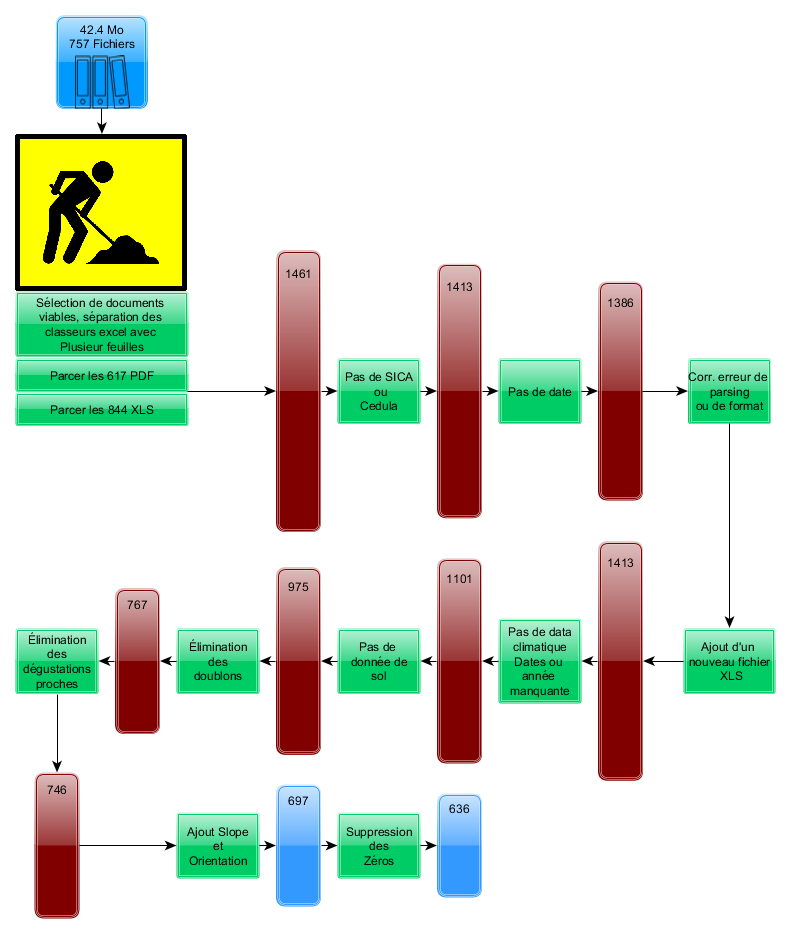
\includegraphics[scale=0.5]{Dataset_2}
	\caption{\label{DatasetMaking} Étape de construction du set de données et pertes d'observations.}
\end{figure}



\paragraph{Variables dépendantes\label{VarDep}} Les variables de sorties, ou dépendantes, sont composées des dix analyses de dégustation et éventuellement de la totalité des défauts physiques des grains. Sauf pour les défauts physiques des grains, qui sont éliminés avant la dégustation, les variables de sorties sont très corrélées entre elles et il a été discuté avec le responsable du comité des caféiculteurs de Risaralda, M. Felipe Rincón, de sélectionner les variables les plus importantes. Ces variables sont \textit{Acidez}, \textit{Dulzor} et \textit{Puntaje Total} ainsi que la catégorie décrite dans le paragraphe suivant qui a été ajouté au set de données.  

\paragraph{Catégories}
Les cafés colombiens sont réputés excellents mais sur les 100 points attribuable lors des dégustations qu'est-ce que cela représente ? Le tableau \ref{categoriesCafe} nous donne une bonne idée de l'échelle de notation. Ces catégories seront utilisées dans le set de données pour tenter de réaliser une classification. 
\begin{table}[H]
	\centering
	\caption{Catégories de cafés d'après le nombre de points \newline Source: http://www.scaa.org/?page=resources\&d=cupping-protocols \label{categoriesCafe}}
	\begin{tabular}{llllcl}
		\textbf{Total Score}   &  & \textbf{Quality Classification}   & \textbf{Specialty or not}  & \textbf{Category} \\
		
		90-100        &  & Outstanding              & Specialty         &  1                    \\
		85-89.99      &  & Excellent                & Specialty         &  2                    \\
		80-84.99      &  & Very Good                & Specialty         &  3                    \\
		\textless80.0 &  & Below Specialty Quality & Not Specialty     &  4                   
	\end{tabular}
\end{table}



\paragraph{Élimination des résultats avec zéro points} Certain cafés du dataset ont zéro points en sortie pour chacune des 10 catégories notées. Il a été décidé de ne pas prendre en compte ces cafés lors des calculs de prédiction ou de clustering car la qualité du sol ou du climat ne peut justifier une telle baisse de qualité à elle seule dans une région réputée propice et qu'un défaut de traitement du grain, un mauvais tri avant la dégustation ou autre facteur externe doit en être la cause. Cependant, afin de se faire une idée d'éventuelles causes de cette qualité médiocre, les cafés sus-mentionnés ont été gardés pour la réalisation des cartes SOM au chapitre \ref{SOM}. 





\subsection{Analyse exploratoire et apprentissage non-supervisé}

\subsubsection{Corrélations entre variables}

Afin d'avoir une bonne vue d'ensemble sur les variables et leurs liens, les matrices de corrélation ont été calculées pour toutes les variables. Premièrement la corrélation entre les différentes sorties. Sur la figure \ref{correlation_sorties1} on peut observer que les défauts physiques des grains ne sont que très peu liés entre eux ou avec les résultats de dégustation. On remarque cependant que les données gustatives du café sont fortement liées entre elles. 

\begin{figure}[H]
	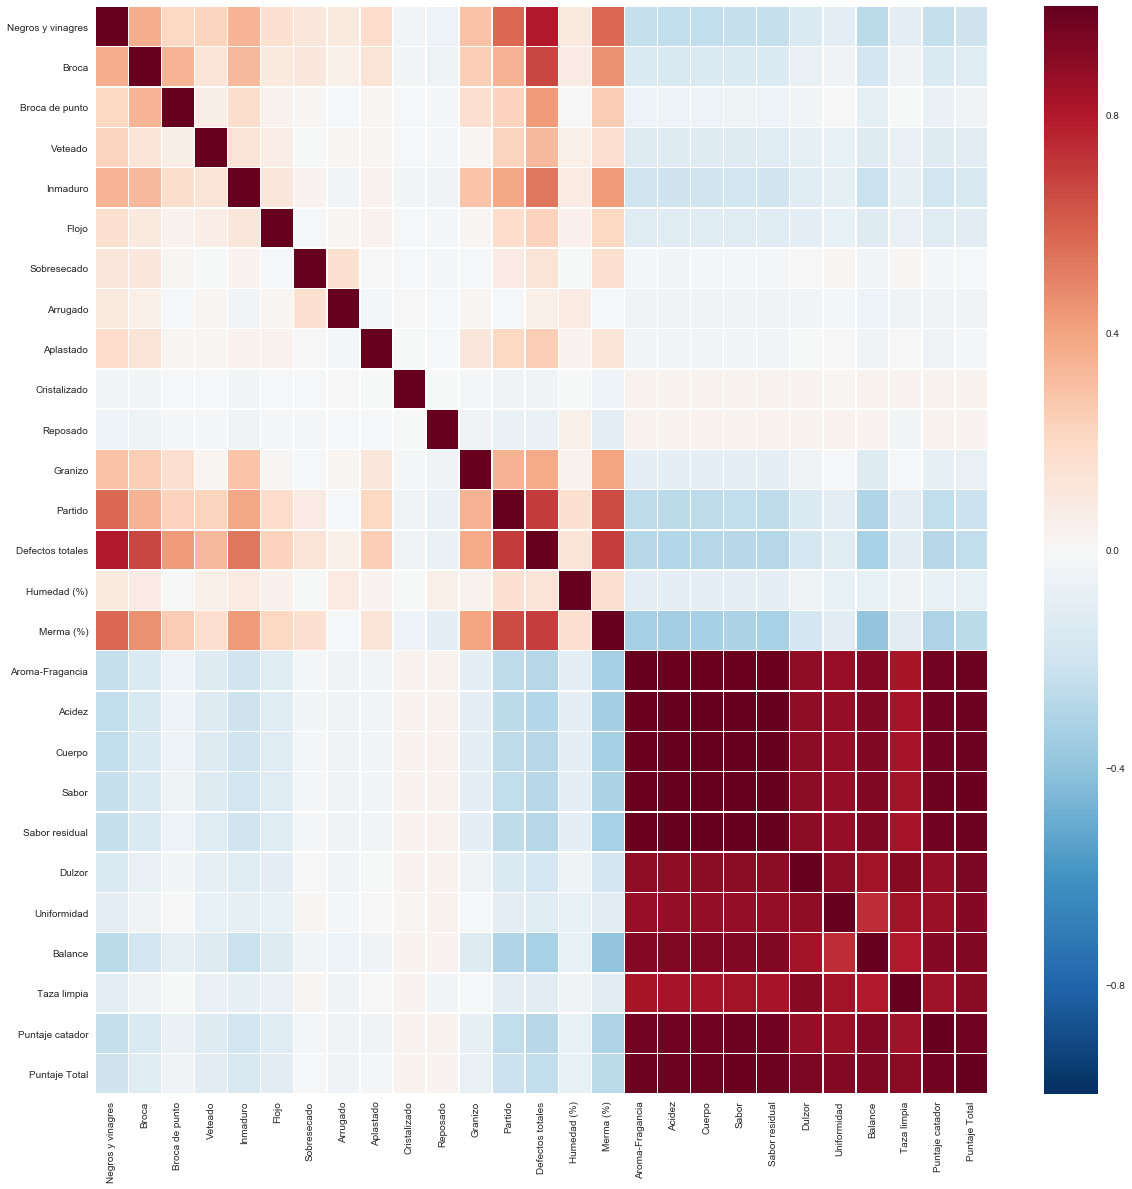
\includegraphics[scale=0.35]{correlation_sorties1}
	\caption{\label{correlation_sorties1} Matrice de corrélation entre les différentes sorties.}
\end{figure}


\noindent Sur la figure \ref{correlation_all1} on peut observer les corrélations entre toutes les variables. 


\begin{figure}[H]
	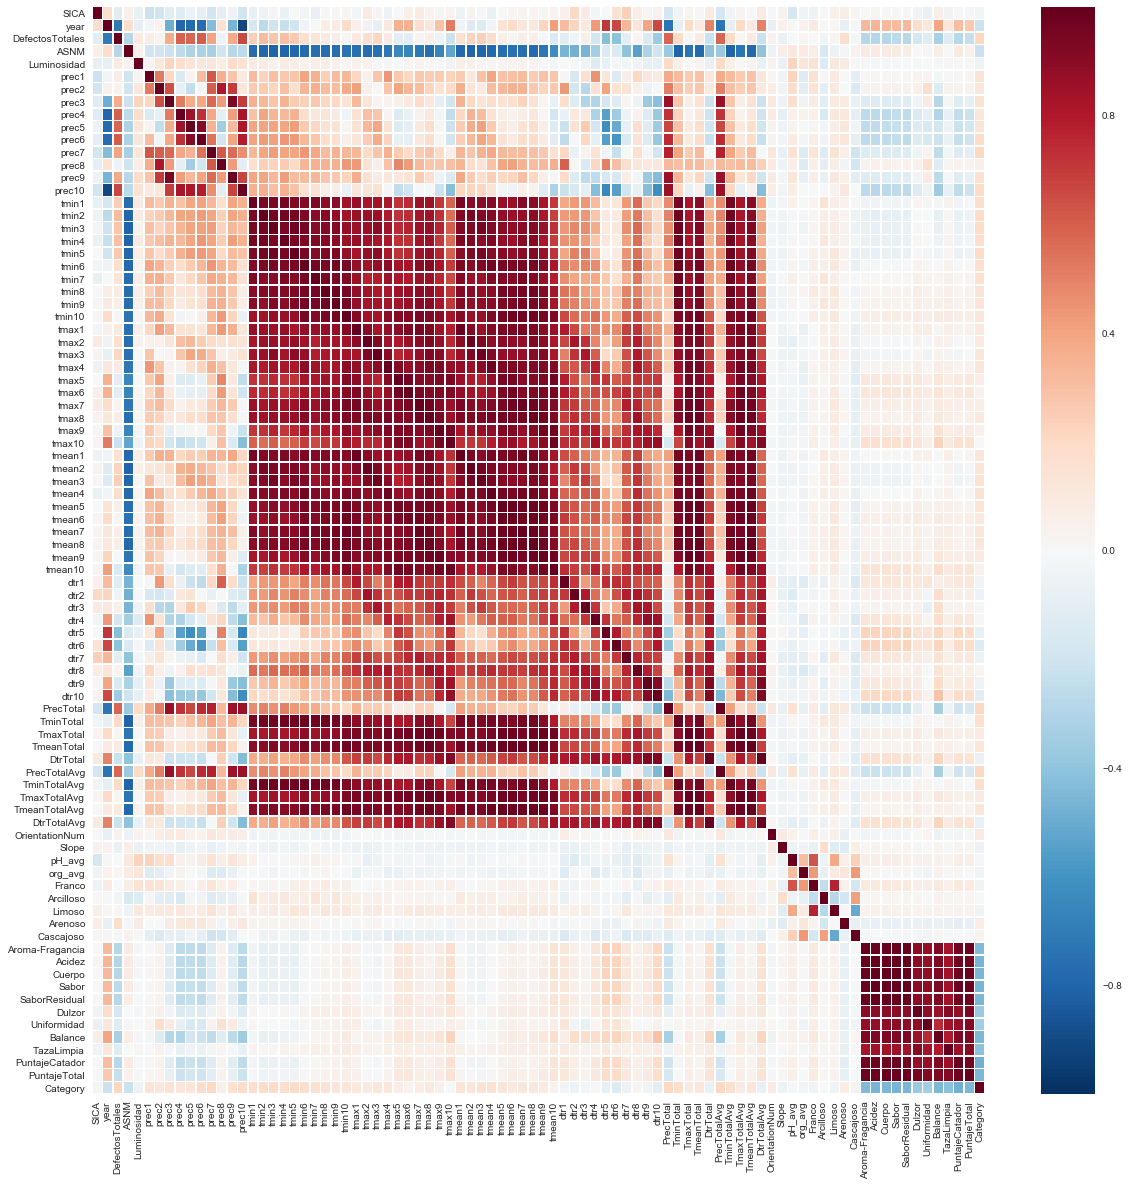
\includegraphics[scale=0.35]{correlation_all1}
	\caption{\label{correlation_all1} Matrice de corrélation entre toutes les variables.}
\end{figure}


\noindent On observe que les données de sol sont parfois corrélées entre-elles mais presque pas du tout avec les données climatiques. On peut donc déjà soulever que le climat n'a pas ou peu d'influence sur la texture, le pH ou le taux de matière organique du sol des zones étudiées. Les précipitations ont une influence importante sur les défauts physiques des grains, en revanche nous n'avons aucune variable qui a une corrélation marquée avec les points totaux et donc la qualité du café.   



%TODO Parler des variétés de cafés et de quelques données les concernants (Moyennes de points, rendement par variété, altitude etc) 
%TODO afficher des moyennes par année etc



\newpage
\subsubsection{Principal Component Analysis (PCA)}\label{PCAss}
La PCA, pour Analyse en Composantes Principales en français, est une méthode qui consiste à transformer un jeu de variables corrélées en nouvelles variables dé-corrélées les unes des autres. Ces nouvelles variables sont appelées composantes principales et permettent de rendre l'information moins redondante. Pour faire plus simple, l'utilité de la Composante Principale est de réduire le nombre de variables tout en gardant un maximum d'information. La figure \ref{PCAdefinition} montre une représentation graphique de la composante principale. 


\begin{figure}[H]
	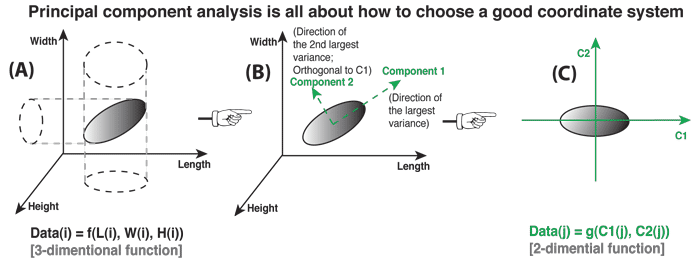
\includegraphics[scale=0.5]{PCA_1}
	\caption{\label{PCAdefinition} Description de l'Analyse en Composante Principale. (A) Description d'un objet simple de manière compliquée ( trois dimensions pour par exemple une ellipse en papier) (B) Trouver des nouvelles variables (axes de coordonnées) orthogonaux l'un à l'autre qui pointent dans les directions de la plus grande variance (C) Utiliser les nouvelles variables (axes) pour décrire l'objet d'une manière plus simple. }
\end{figure}

\paragraph{Résultats de la PCA}

L'analyse sur une version compacte des variables a donné les résultats présentés dans le tableau \ref{TablePCAResult1} et sur la figure \ref{FigurePCAResult1}. Une première analyse avait été effectuée sur le set de données complet, c'est-à-dire avec la totalité des données climatiques et non les moyennes, et les résultats se sont avérés similaires mais plus difficilement lisibles. Il a donc été choisi de résumer les variables pour réaliser la PCA et le clustering. La PCA du tableau \ref{TablePCAResult1} ne comprend pas les cafés avec zéro points.
\begin{table}[]
	\centering
	\begin{tabular}{lllllll}
		& PC1     & PC2     & PC3     & PC4     & PC5     & PC6     \\
		ASNM           & \textbf{0.4125}  & 0.0766  & -0.0360 & 0.1766  & -0.1337 & 0.0397  \\
		Luminosidad    & -0.0169 & 0.2320  & 0.1532  & -0.3178 & -0.2836 & 0.0157  \\
		PrecTotalAvg   & -0.1714 & 0.1424  & 0.0222  & \textbf{-0.6767} & -0.0667 & 0.0926  \\
		TminTotalAvg   & \textbf{-0.4589} & -0.0115 & 0.1086  & -0.1232 & 0.0013  & 0.0809  \\
		TmaxTotalAvg   & \textbf{-0.4745} & -0.0334 & 0.0296  & 0.1501  & -0.0253 & -0.0329 \\
		TmeanTotalAvg  & \textbf{-0.4803} & -0.0252 & 0.0631  & 0.0409  & -0.0149 & 0.0133  \\
		DtrTotalAvg    & -0.3323 & -0.0517 & -0.0884 & \textbf{0.4712}  & -0.0529 & -0.1769 \\
		OrientationNum & 0.0623  & 0.0592  & -0.0886 & -0.1839 & \textbf{0.3797}  & \textbf{-0.5662} \\
		Slope          & 0.0657  & -0.1842 & 0.1179  & 0.1047  & 0.0434  & \textbf{0.6905}  \\
		pH\_avg        & 0.0135  & 0.3892  & 0.3844  & -0.0168 & 0.1244  & 0.0679  \\
		org\_avg       & 0.0493  & 0.1781  & \textbf{0.5036}  & 0.2176  & -0.1639 & -0.1841 \\
		Franco         & -0.0157 & \textbf{0.5453}  & 0.1441  & 0.1921  & 0.1676  & 0.1108  \\
		Arcilloso      & -0.0180 & -0.3026 & 0.2993  & -0.0844 & \textbf{0.4532}  & 0.1751  \\
		Limoso         & -0.0754 & \textbf{0.5018}  & \textbf{-0.2016} & 0.1095  & 0.2726  & 0.1712  \\
		Arenoso        & -0.0210 & 0.0645  & 0.0180  & 0.0048  & \textbf{-0.6303} & -0.0156 \\
		Cascajoso      & 0.0760  & -0.2236 & \textbf{0.6130}  & 0.0095  & 0.0109  & \textbf{-0.2053}
	\end{tabular}
	\caption{\label{TablePCAResult1}Tableau des rotations des six premiers composants de la PCA avec mise en évidence des variables les plus importantes par composante.}
\end{table}


\begin{figure}[H]
	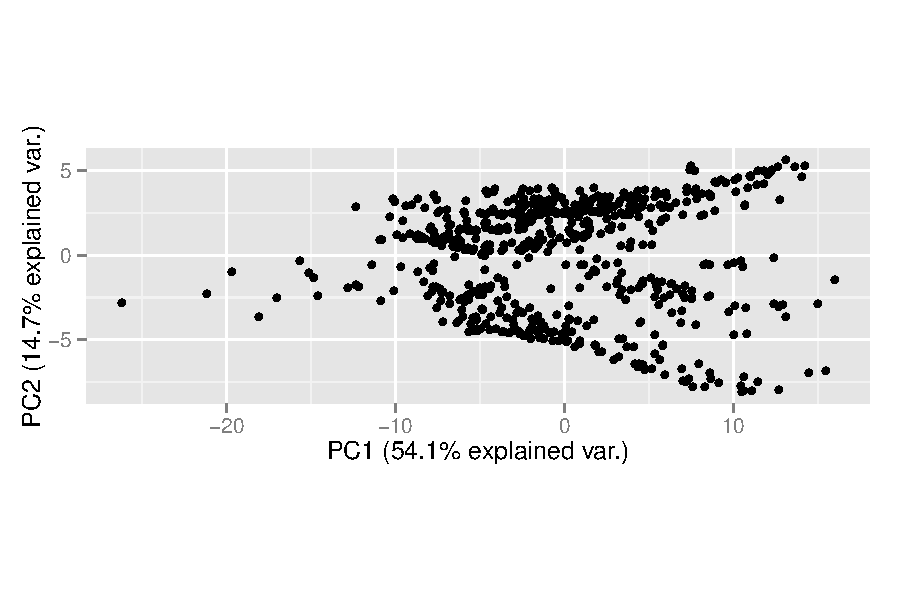
\includegraphics[scale=1]{pca_complete.pdf}
	\caption{\label{FigurePCAResult1} Résultats de la PCA sous forme graphique. Réalisé avec la totalité des variables }
\end{figure}


\paragraph{Analyse des composantes} Le tableaux \ref{TablePCAResult1} montre l'importance des variables dans les différentes composantes de la PCA réalisée avec un  jeu de variables simplifié pour plus de lisibilité, après vérification que l'importance des types de variables des deux tableaux était similaire. \\

\noindent La première composante met en évidence les températures par rapport à l'altitude alors que la deuxième et la troisième mettent en évidence principalement les caractéristiques du sol. La quatrième montre une dé-corrélation entre les précipitations moyennes et les DTR et la cinquième composante montre une corrélation entre la texture argileuse du sol et son orientation à l'opposé à d'un sol sablonneux. La sixième composante met en évidence une relation entre l'orientation et et les sols rocailleux à l'opposé des sols pentus. 


\paragraph{PCA avec prcomp} Afin de visualiser au mieux les données dans la PCA, une autre PCA a été réalisée àl'aide d'un autre outil (prcomp) et chaque point a été coloré selon son année (figure \ref{fig:pcayear}) ou selon sa catégorie (figure \ref{fig:pcacat}). 


\begin{figure}[H]
	\centering
	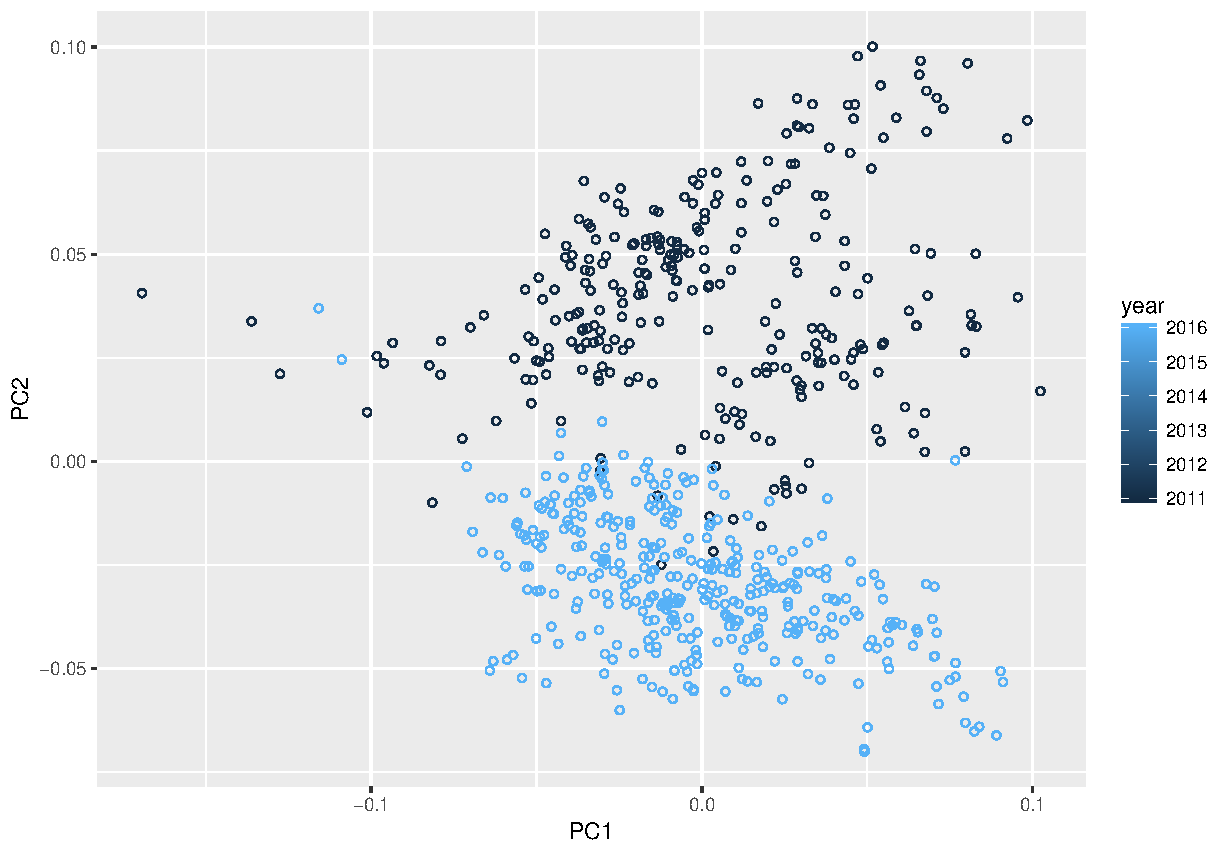
\includegraphics[width=0.7\linewidth]{img/PCA/PCAYear}
	\caption{PCA avec Prcomp: Coloration par année}
	\label{fig:pcayear}
\end{figure}


\begin{figure}[H]
	\centering
	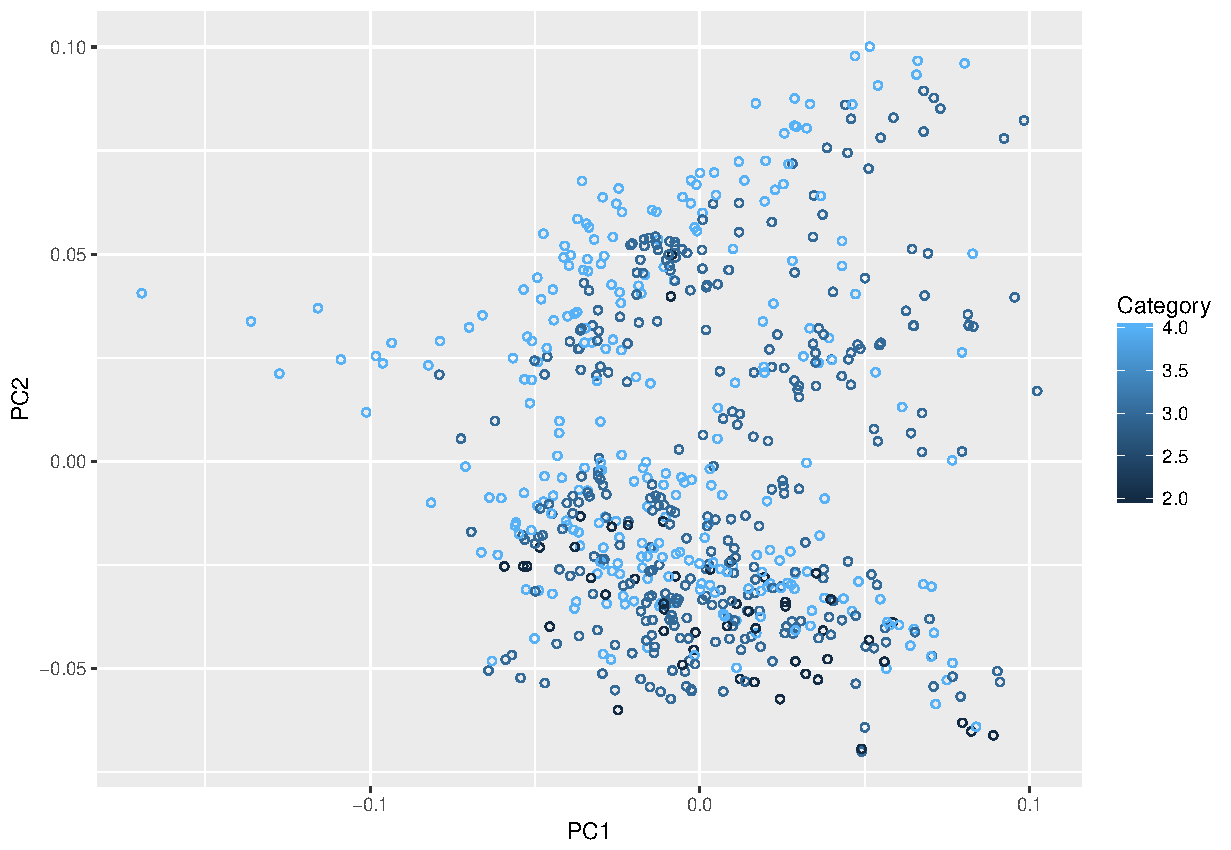
\includegraphics[width=0.7\linewidth]{img/PCA/PCACat}
	\caption{PCA avec Prcomp: Coloration par catégorie}
	\label{fig:pcacat}
\end{figure}





\noindent On peut observer que les deux années sont bien différenciées. Les premiers composants de la PCA montrent l'importance des variables climatiques et les différences entre années sont visibles sur ces graphiques. Les catégories sont aussi différemment réparties. En retournant sur les moyennes de chaque année (Voir description des données section \ref{YearlyPuntajeTotal}), on peut voir que l'année 2011 possède en effet moins de café en nombre mais plus de cafés ayant reçu la note de zéro. On peut aussi voir que les conditions climatiques sont différentes entre les deux années, surtout en termes de précipitations. La section \ref{SOM} montre les relations entre le climat et les défauts totaux, qui peuvent influencer la qualité finale du café.  %TODO
% https://georgemdallas.wordpress.com/2013/10/30/principal-component-analysis-4-dummies-eigenvectors-eigenvalues-and-dimension-reduction/

%https://onlinecourses.science.psu.edu/stat505/node/54
\newpage
\subsubsection{Clustering} Afin de vérifier la présence éventuelle de groupes d'individus parmi la population de café, nous réalisons un HCPC, pour \textit{Hierarchical Clustering on Principal Components}, à l'aide de la PCA. La figure \ref{HCTSuggest} nous montre l'arbre hiérarchique créé ainsi que le nombre de cluster proposé. \\

\begin{figure}[H]
	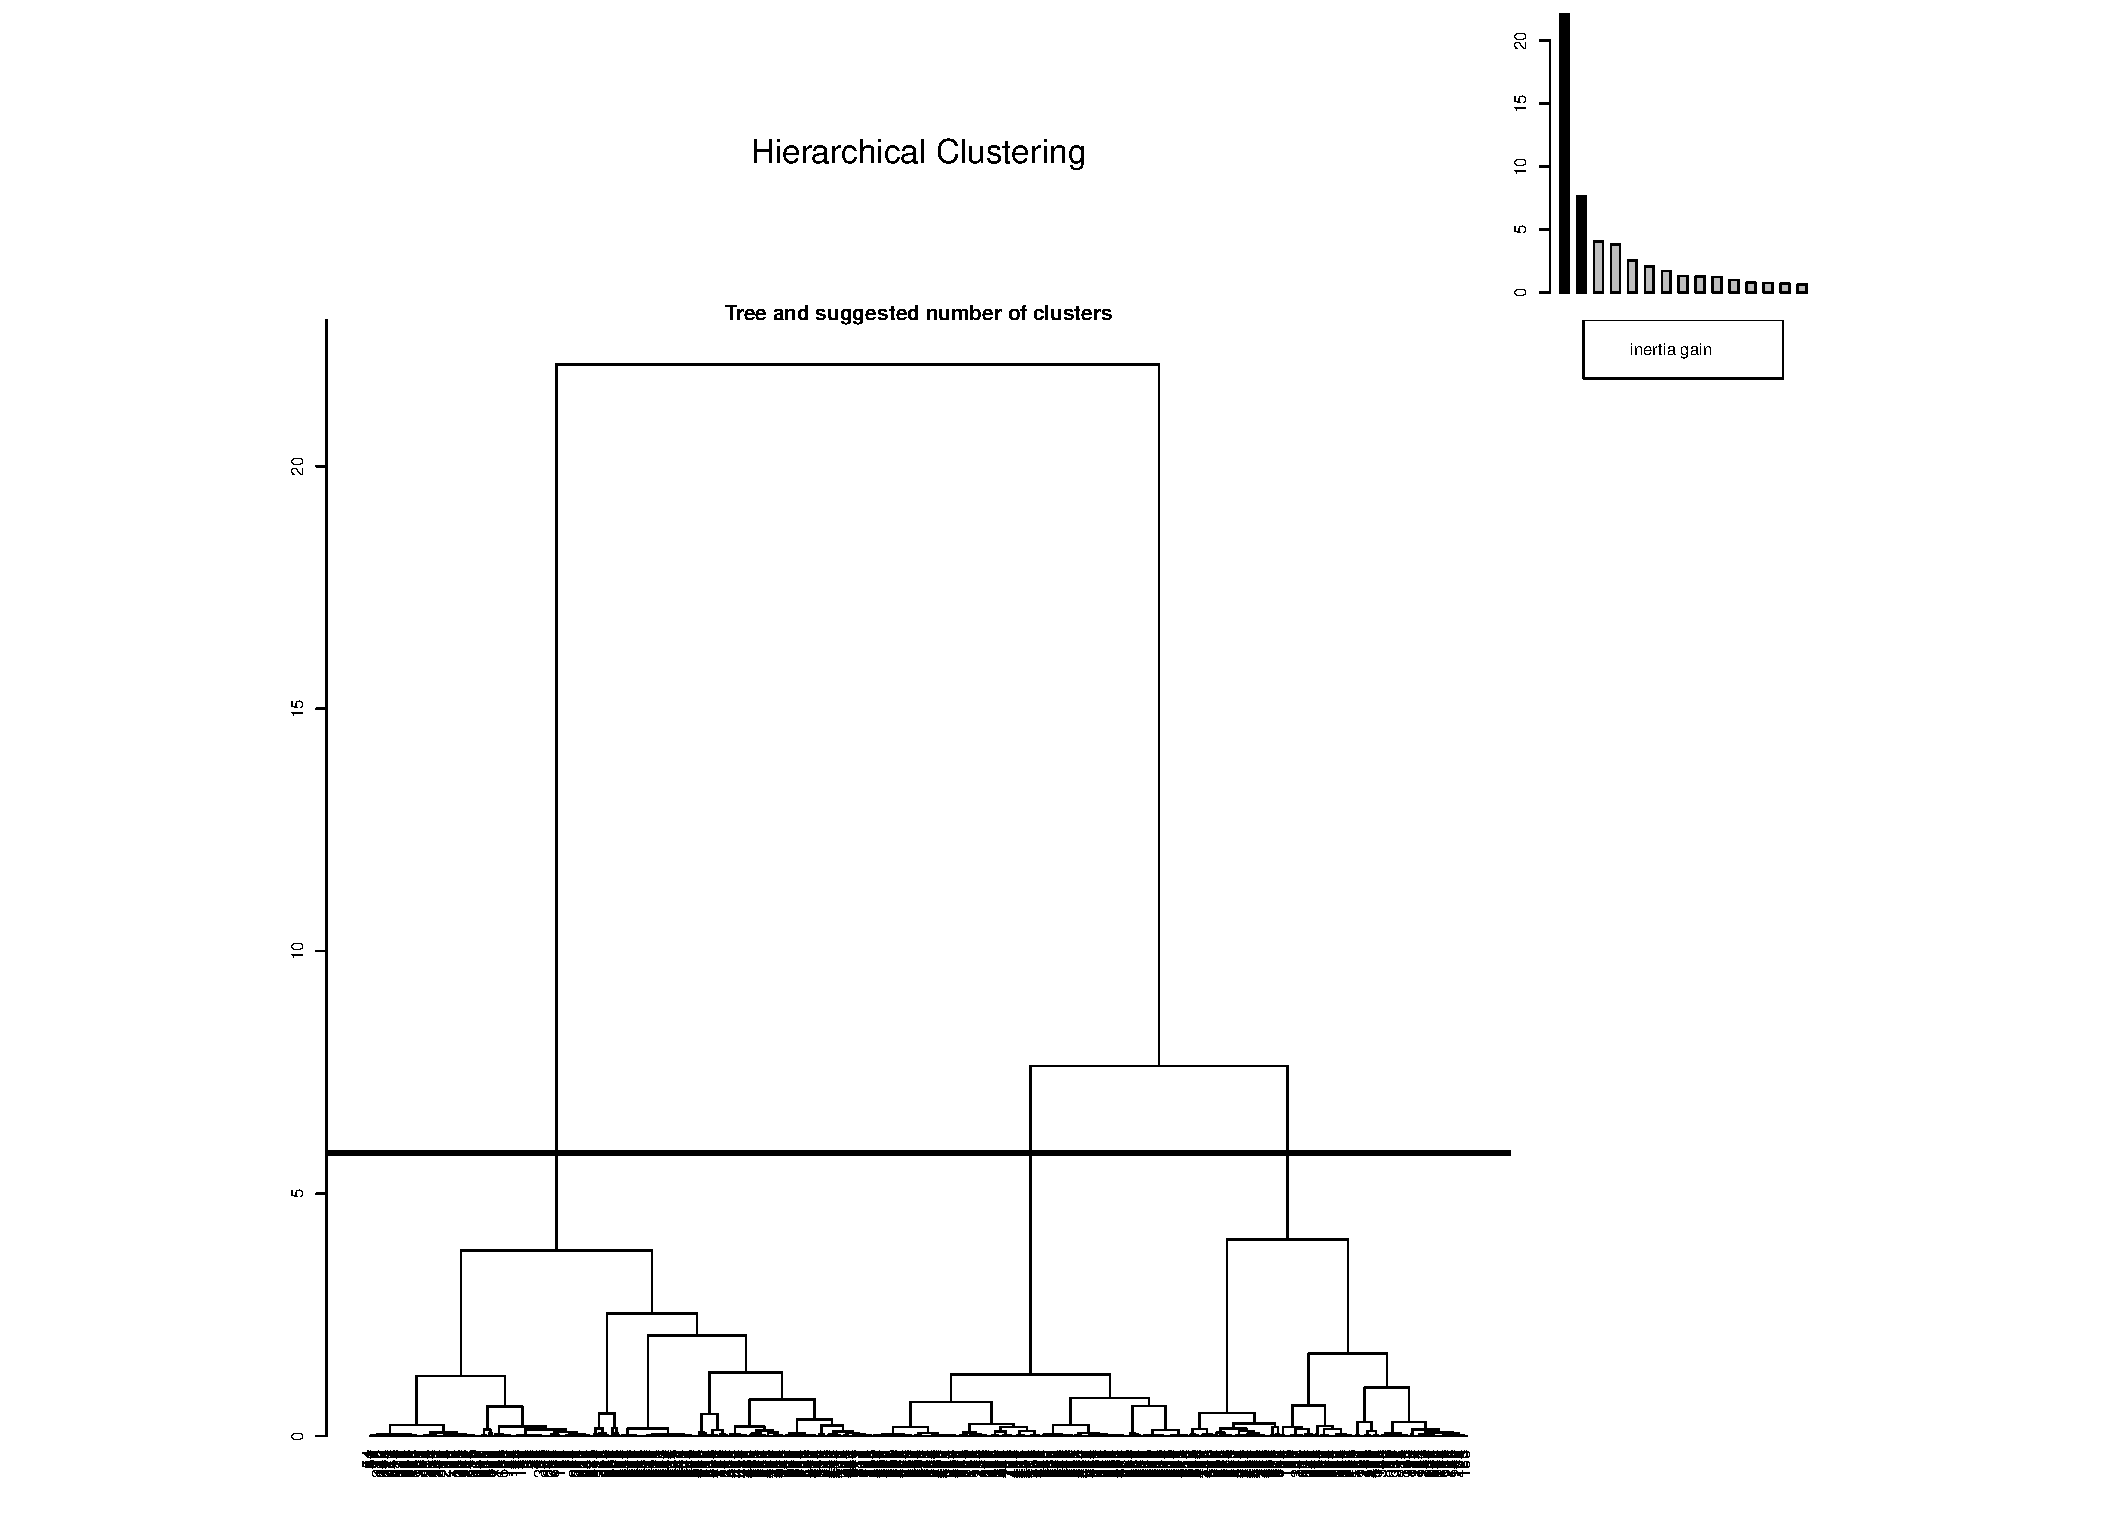
\includegraphics[scale=0.45]{HierarchicalClustering_TreeAndSuggestedNbCluster.pdf}
	\caption{\label{HCTSuggest} HCPC et proposition de nombre de cluster }
\end{figure}

\noindent La figure \ref{HCT_3d} montre une représentation du HCPC en 3D. On reconnais la forme de la PCA mais les clusters sont plutôt décevants car le découpage je fais pas ressortir les groupes éventuellement visibles. Comme on l'a vu précédemment, avec la PCA et les différentes moyennes, les deux années sont très différentes et on aurait pu s'attendre à un clustering plus efficace. 

\begin{figure}[H]
	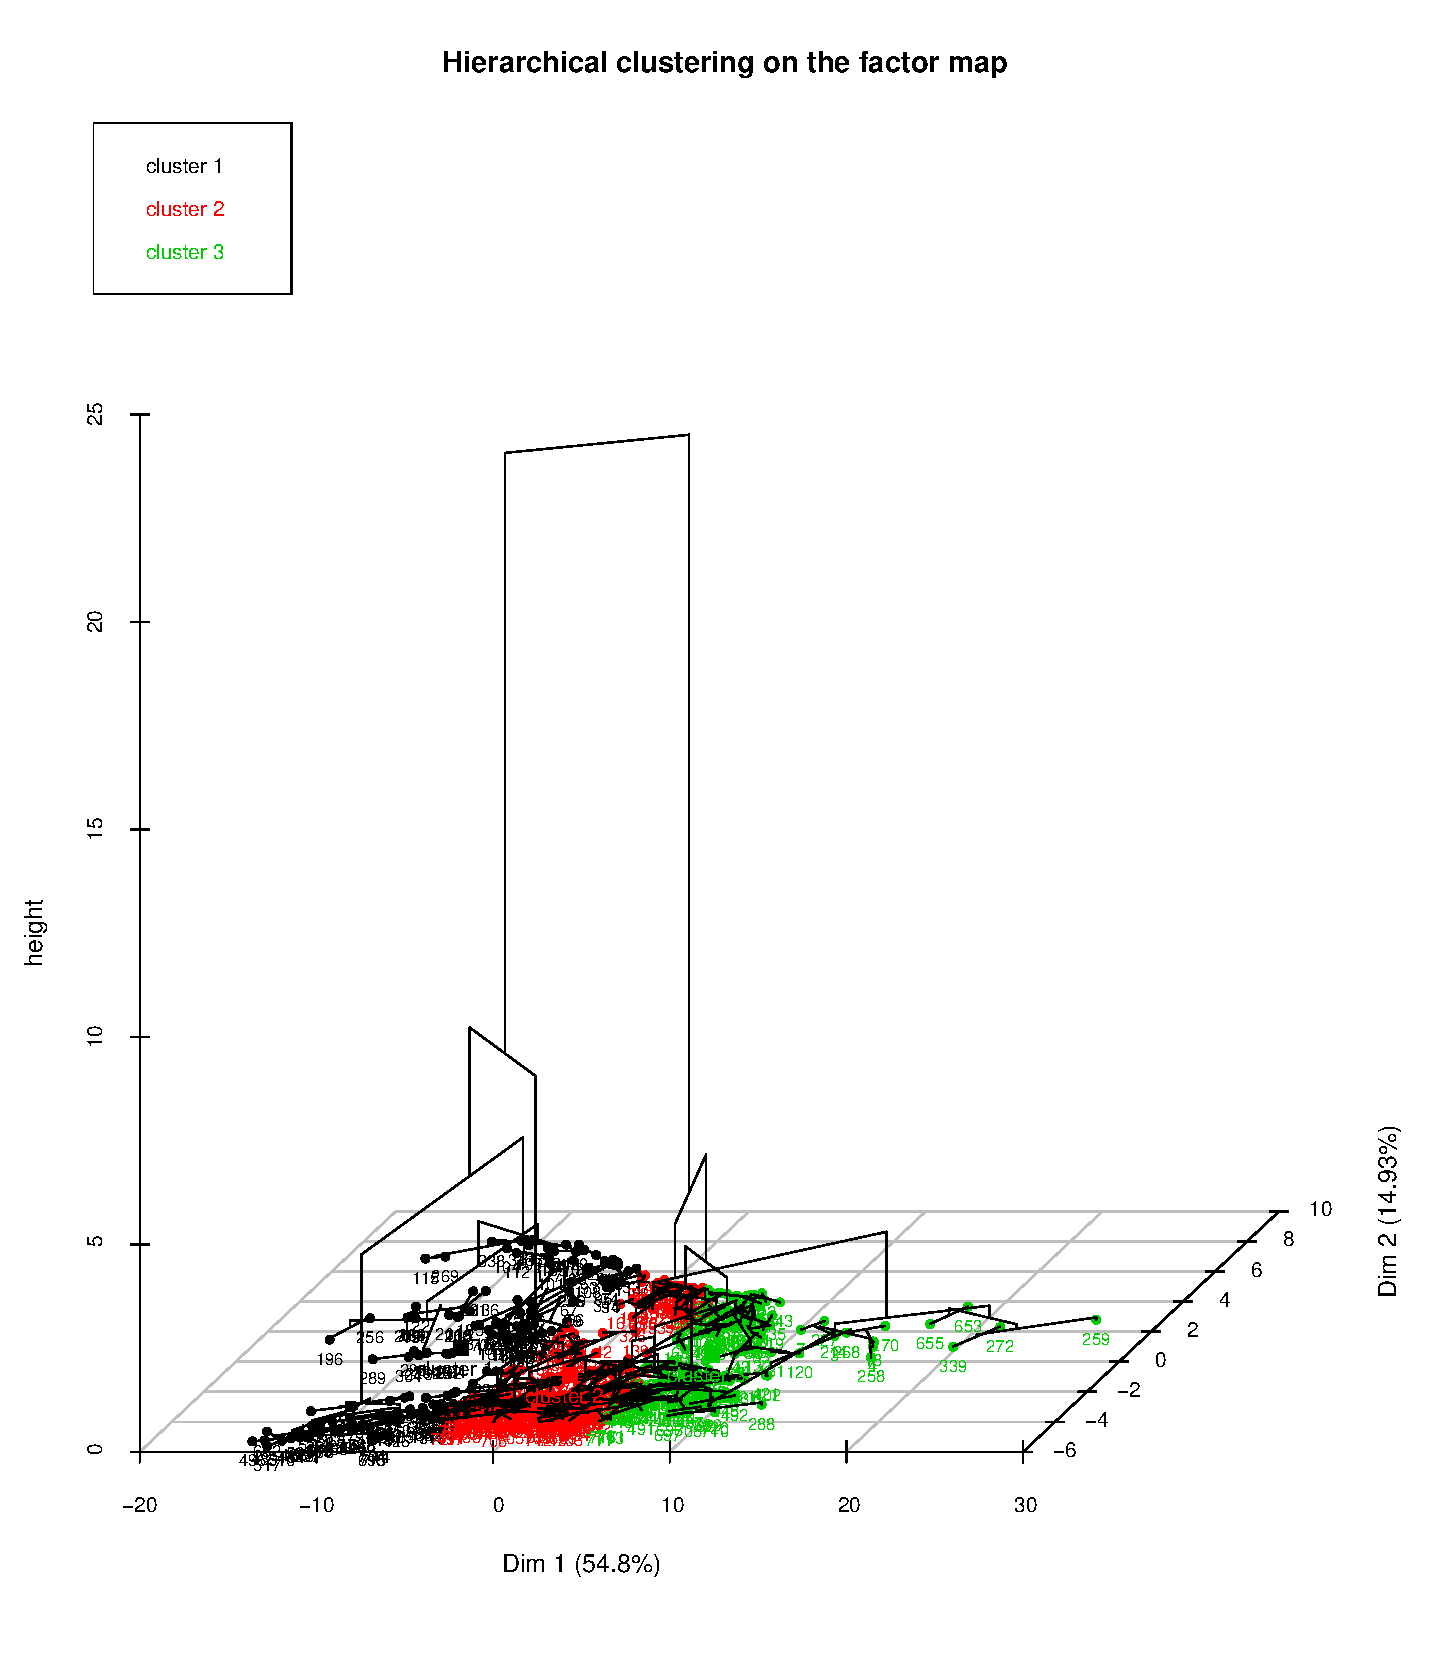
\includegraphics[scale=0.6]{HierarchicalClustering3D.pdf}
	\caption{\label{HCT_3d} HCPC arbre 3D}
\end{figure}


\noindent La figure \ref{HCT_Inert} nous montre les sauts d'inertie du dendogramme. On peut y voir qu'entre 2 et 3 clusters nous avons un saut assez grand puis à nouveau entre 4 et 5 avant une stabilisation. 


%http://www.sthda.com/english/wiki/hcpc-hierarchical-clustering-on-principal-components-hybrid-approach-2-2-unsupervised-machine-learning

\begin{figure}[H]
	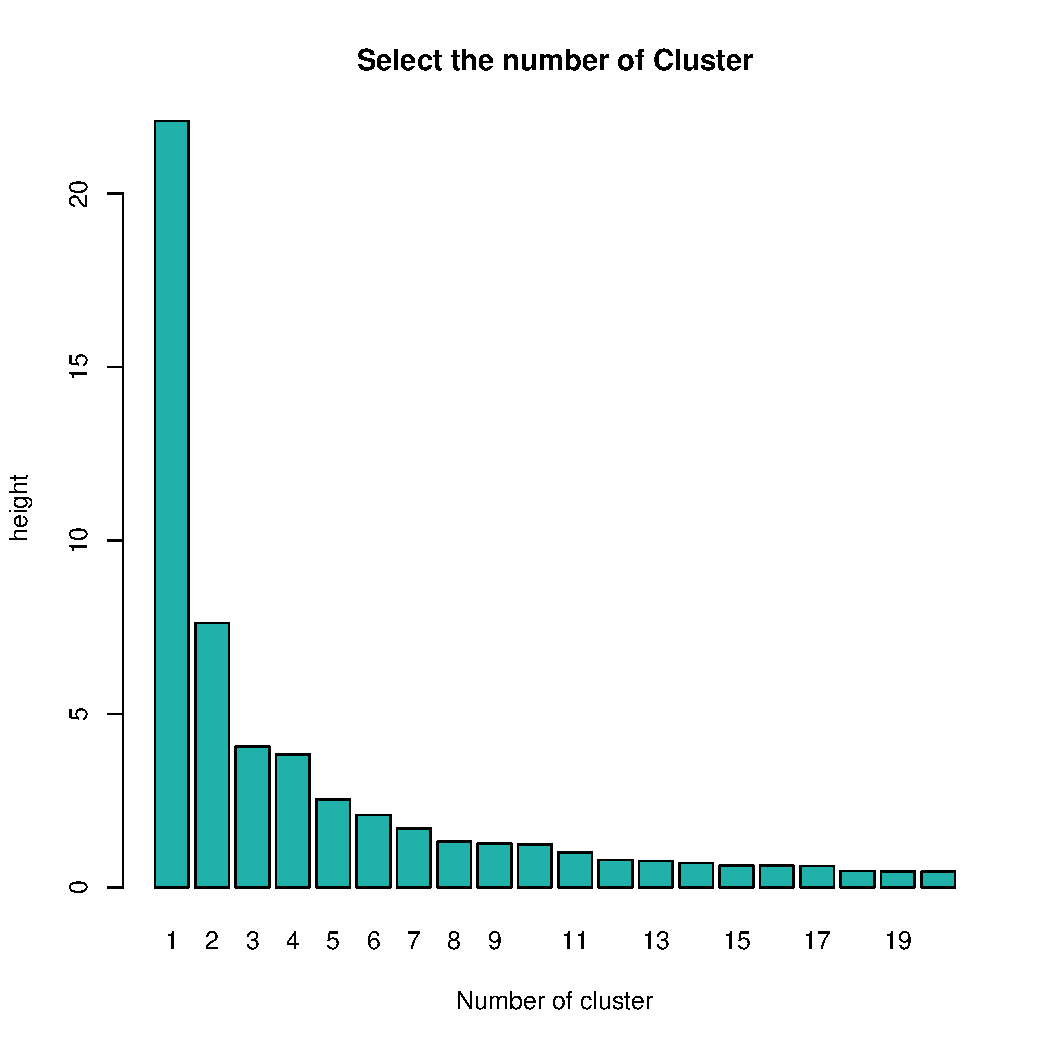
\includegraphics[scale=0.55]{NbClusterSelectInertiaGain.pdf}
	\caption{\label{HCT_Inert} Saut d'inertie du dendogramme  }
\end{figure}

%\noindent L'outil de HCPC nous fournit en sortie un objet de description des classes par les variables





\noindent L'ajout de clusters au set de données serait utile du moment que les clusters permettent significativement de séparer les types de cafés, au sens variables dépendantes du terme. Visuellement on devrait pouvoir observer une différence entre le nombre de café dans chaque cluster et les variables de sorties. Cependant ce n'est pas le cas comme on peut le voir ci-dessous: 


\begin{table}[H]
	\centering
	\label{cluster3category}
	\begin{tabular}{llll}
		 & 1  & 2  & 3   \\
		 \hline
		cat 2            & 0  & 28 & 21  \\
		cat 3            & 72 & 98 & 146 \\
		cat 4            & 44 & 70 & 157 
	\end{tabular}
	\caption{HCPC avec trois clusters comparés à la sortie catégories}
\end{table}


\noindent Les autres résultats ainsi que l'importance des variables pour la génération des clusters se trouvent dans l'annexe \ref{annexe:clust}.\\


\noindent Les variables participent presque toute activement à la séparation en partie (en prenant en compte les 5\% de probabilité critiques ) cependant la séparation n'apporte rien au set de donnée puis-qu'elle ne sépare en rien les différents types de cafés (note basse - note haute).



%\paragraph{Analyse des résultats de clustering}
%TODO - vérifier






















\newpage
\subsubsection{Self-Organizing Map}\label{SOM}
%TODO 

\paragraph{U-Matrix, répartition des cafés par classes et composants} 
La carte auto-organisatrice a été réalisée en incluant toutes les variables afin de voir où se placent les variables dépendantes par rapport aux variables indépendantes et de permettre d'observer d'éventuels clusters. 


\begin{figure}[H]
	\centering
	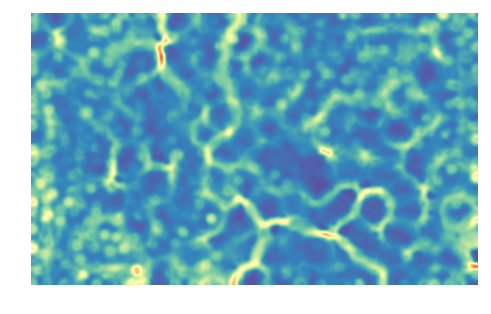
\includegraphics[width=0.7\linewidth]{SOM/SOM_Umatrix}
	\caption{U-Matrix de la carte SOM}
	\label{}
\end{figure}

\begin{figure}[H]
	\centering
	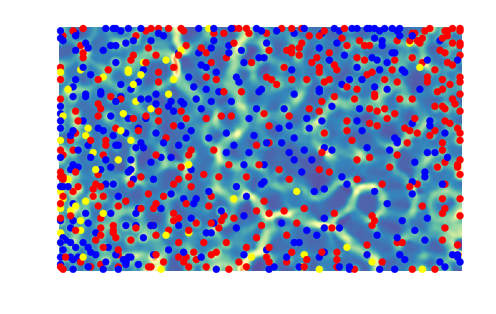
\includegraphics[width=1\linewidth]{SOM/SOM_Umatrix_Points_Category}
	\caption{\label{umatrix_cat}U-Matrix avec les points. En jaune les cafés de catégorie 2,en bleu catégorie 3 et en rouge catégorie 4. Les catégories sont expliquées au point \ref{EmpFermes}}
	\label{}
\end{figure}


\begin{figure}[H]
	\caption{Composants de qualité - Variables de sortie}
	\centering
		\subfloat[Acidez]{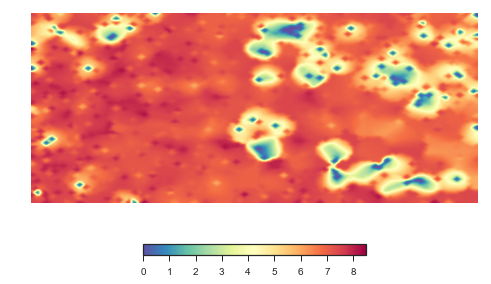
\includegraphics[width=.3\linewidth]{SOM/SOM_Acidez}}\hfill
		\subfloat[Aroma-Fragrancia]{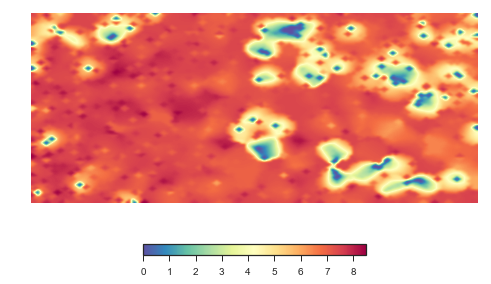
\includegraphics[width=.3\linewidth]{SOM/SOM_AromaFragrancia}}\hfill
		\subfloat[Cuerpo]{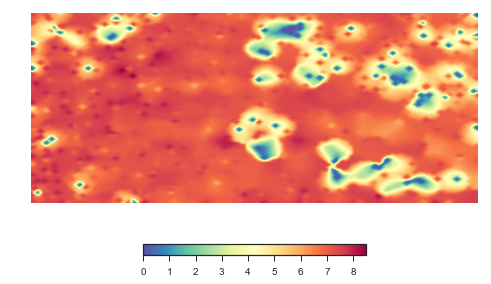
\includegraphics[width=.3\linewidth]{SOM/SOM_Cuerpo}}
		\newline
		\subfloat[Balance]{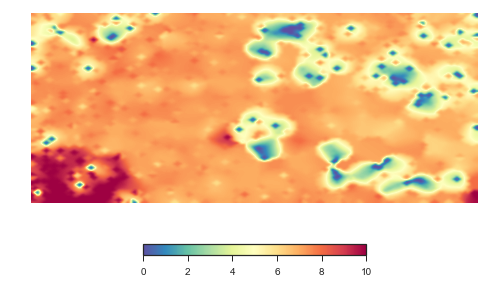
\includegraphics[width=.3\linewidth]{SOM/SOM_Balance}}\hfill
		\subfloat[Uniformidad]{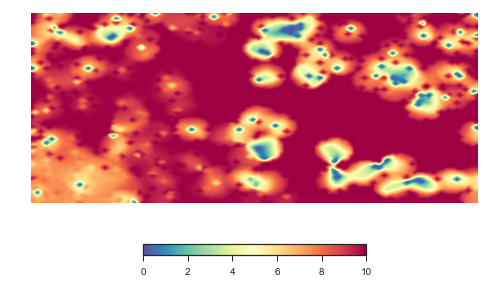
\includegraphics[width=.3\linewidth]{SOM/SOM_Uniformidad}}\hfill
		\subfloat[Taza Limpia]{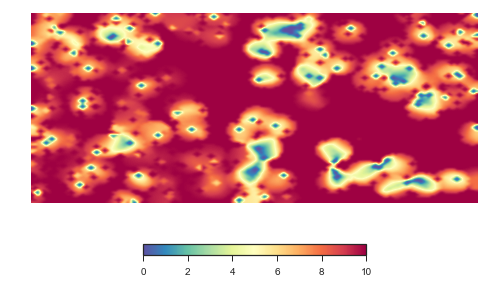
\includegraphics[width=.3\linewidth]{SOM/SOM_TazaLimpia}}
		\newline
		\subfloat[Dulzor]{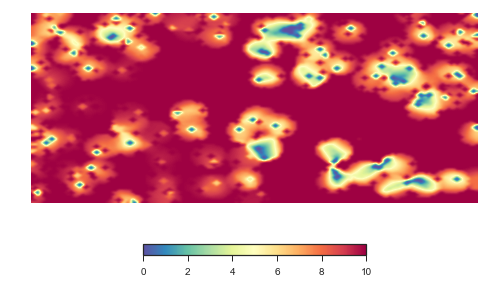
\includegraphics[width=.3\linewidth]{SOM/SOM_Dulzor}}\hfill
		\subfloat[Sabor]{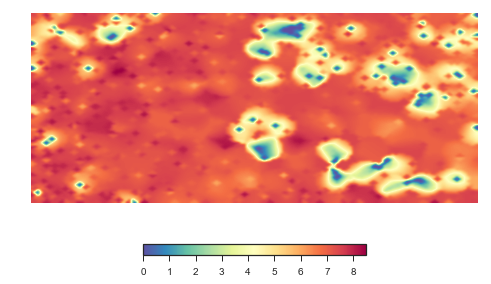
\includegraphics[width=.3\linewidth]{SOM/SOM_Sabor}}\hfill
		\subfloat[Sabor Residual]{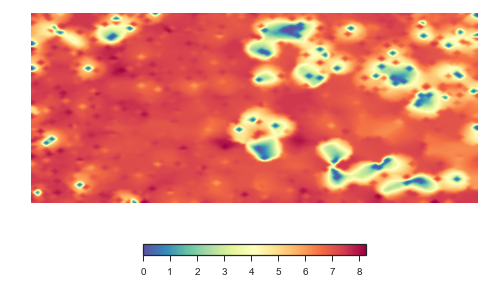
\includegraphics[width=.3\linewidth]{SOM/SOM_SaborResidual}}
		\newline
		\centering
		\subfloat[Puntaje Catador]{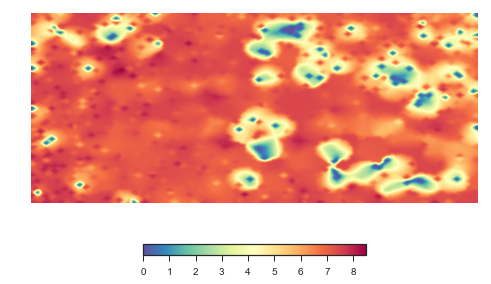
\includegraphics[width=.3\linewidth]{SOM/SOM_PuntajeCatador}}\hfill
		\subfloat[Puntaje Total]{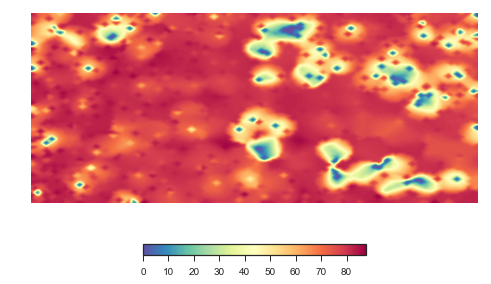
\includegraphics[width=.3\linewidth]{SOM/SOM_PuntajeTotal}}
\end{figure}




\begin{figure}[H]
	\caption{Précipitations}
	\centering
	\subfloat[Prec1]{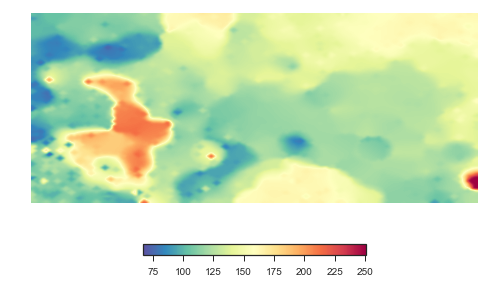
\includegraphics[width=.3\linewidth]{SOM/SOM_Prec1}}\hfill
	\subfloat[Prec2]{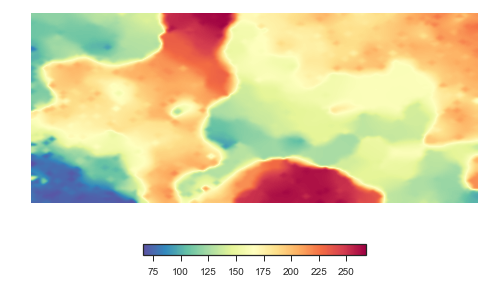
\includegraphics[width=.3\linewidth]{SOM/SOM_Prec2}}\hfill
	\subfloat[Prec3]{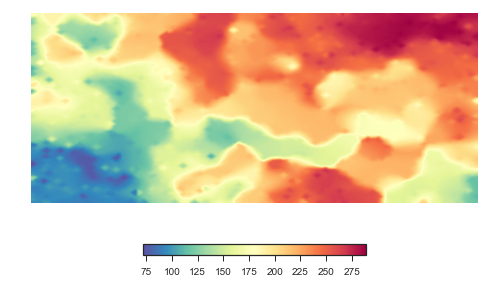
\includegraphics[width=.3\linewidth]{SOM/SOM_Prec3}}\hfill
	\newline
	\subfloat[Prec4]{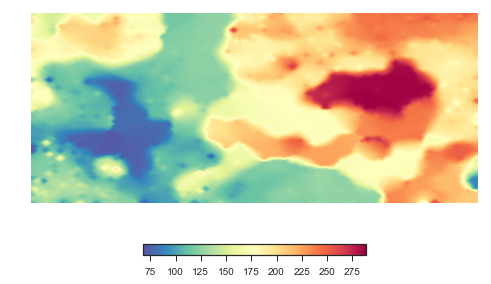
\includegraphics[width=.3\linewidth]{SOM/SOM_Prec4}}\hfill
	\subfloat[Prec5]{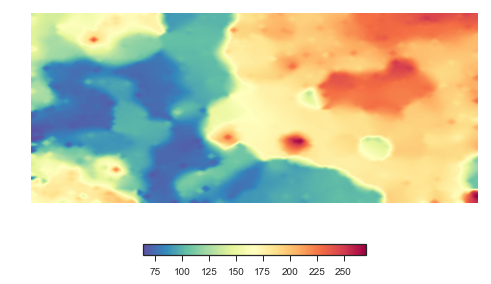
\includegraphics[width=.3\linewidth]{SOM/SOM_Prec5}}\hfill
	\subfloat[Prec6]{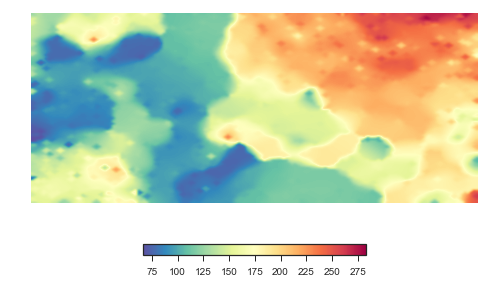
\includegraphics[width=.3\linewidth]{SOM/SOM_Prec6}}\hfill
	\newline
	\subfloat[Prec7]{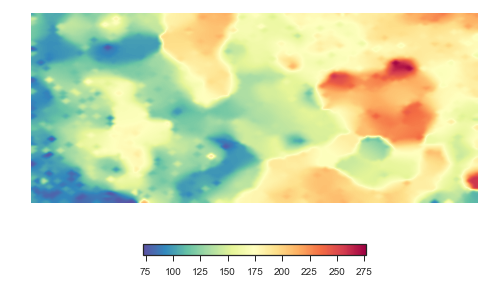
\includegraphics[width=.3\linewidth]{SOM/SOM_Prec7}}\hfill
	\subfloat[Prec8]{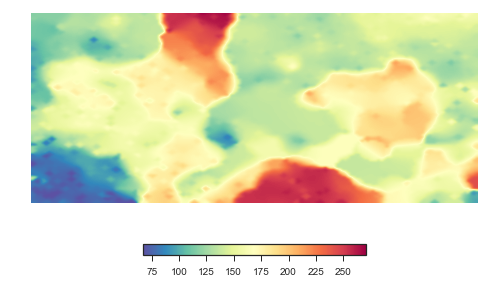
\includegraphics[width=.3\linewidth]{SOM/SOM_Prec8}}\hfill
	\subfloat[Prec9]{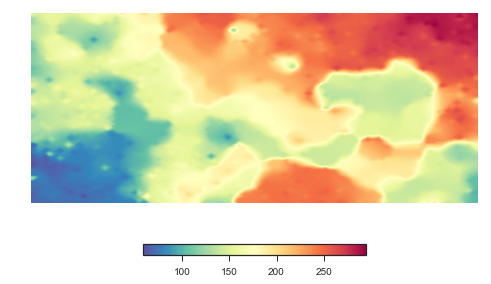
\includegraphics[width=.3\linewidth]{SOM/SOM_Prec9}}\hfill
	\newline
	\centering
	\subfloat[Prec10]{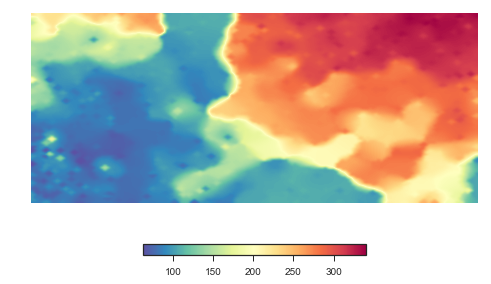
\includegraphics[width=.3\linewidth]{SOM/SOM_Prec10}}
	\subfloat[Average]{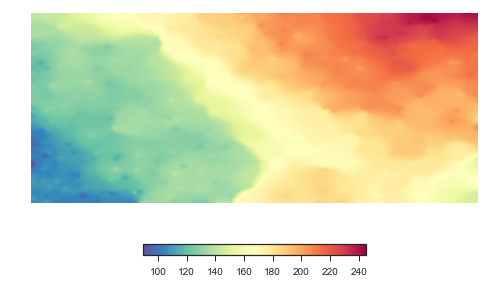
\includegraphics[width=.3\linewidth]{SOM/SOM_PrecTotalAvg}}
\end{figure}



\begin{figure}[H]
	\caption{SOM - Autres données}
	\centering
	\subfloat[Temp. Min. Average]{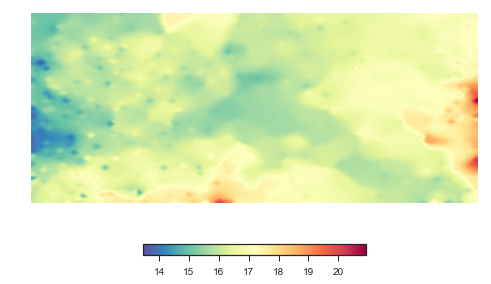
\includegraphics[width=.3\linewidth]{SOM/SOM_TminTotalAvg}}\hfill
	\subfloat[Temp. Max. Average]{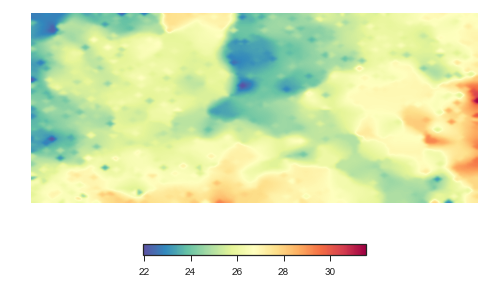
\includegraphics[width=.3\linewidth]{SOM/SOM_TmaxTotalAvg}}\hfill
	\subfloat[Temp. Mean. Average]{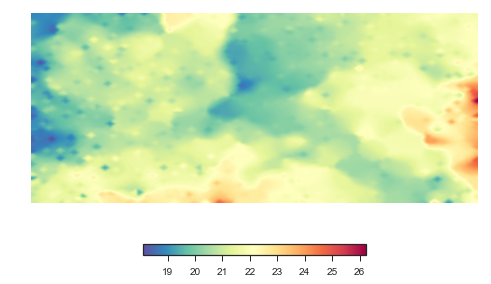
\includegraphics[width=.3\linewidth]{SOM/SOM_TmeanTotalAvg}}\hfill
	\newline
	\subfloat[Dtr Average]{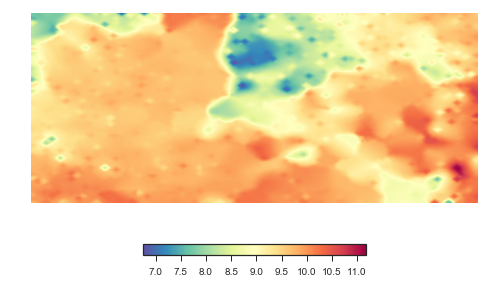
\includegraphics[width=.3\linewidth]{SOM/SOM_DtrTotalAvg}}\hfill
	\subfloat[ASNM]{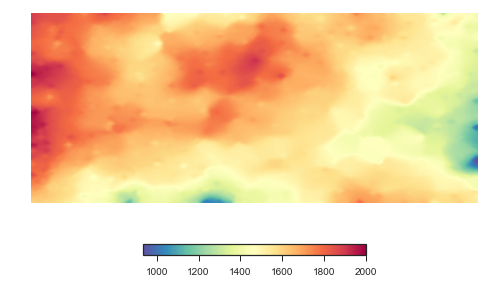
\includegraphics[width=.3\linewidth]{SOM/SOM_ASNM}}\hfill
	\subfloat[Slope]{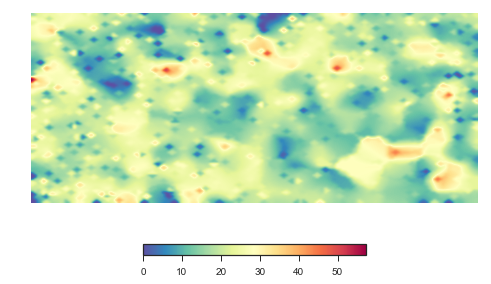
\includegraphics[width=.3\linewidth]{SOM/SOM_Slope}}\hfill
	\newline
	\subfloat[Franco]{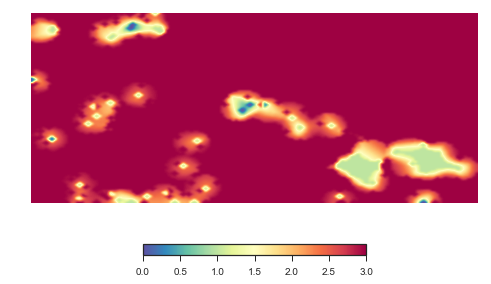
\includegraphics[width=.3\linewidth]{SOM/SOM_Franco}}\hfill
	\subfloat[Arenoso]{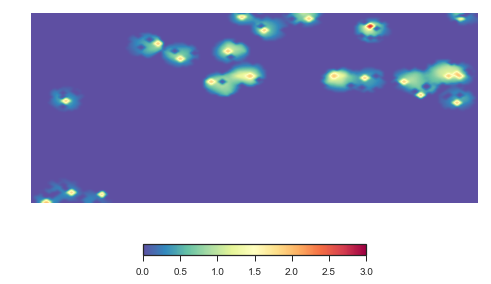
\includegraphics[width=.3\linewidth]{SOM/SOM_Arenoso}}\hfill
	\subfloat[Arcilloso]{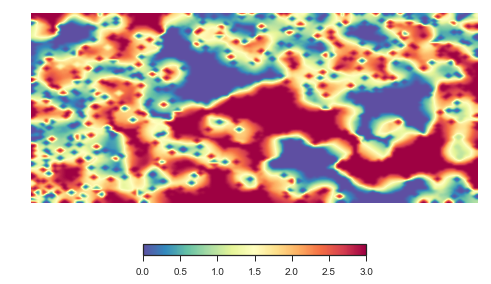
\includegraphics[width=.3\linewidth]{SOM/SOM_Arcilloso}}\hfill
	\newline
	\centering
	\subfloat[Limoso]{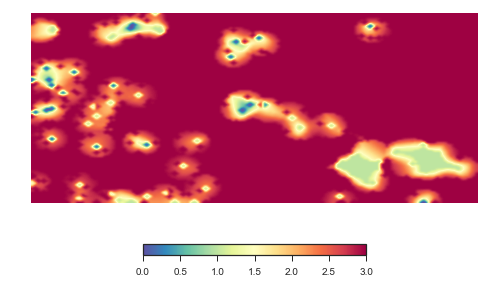
\includegraphics[width=.3\linewidth]{SOM/SOM_Limoso}}\hfill
	\subfloat[Cascajoso]{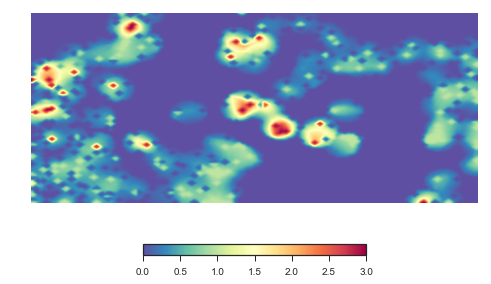
\includegraphics[width=.3\linewidth]{SOM/SOM_Cascajoso}}\hfill
	\subfloat[pH]{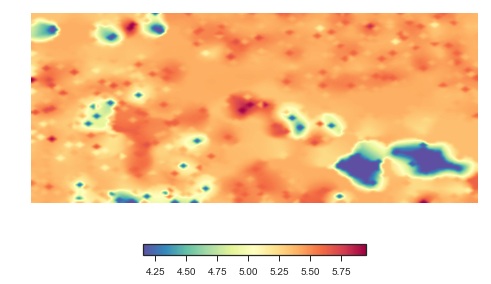
\includegraphics[width=.3\linewidth]{SOM/SOM_pHAvg}}\hfill
	\newline
	\subfloat[Organic]{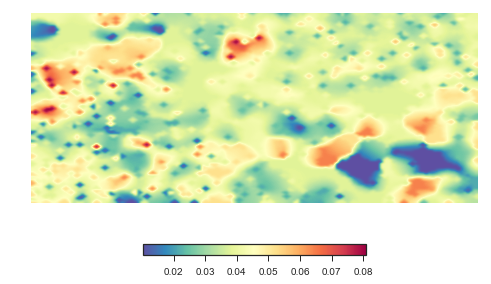
\includegraphics[width=.3\linewidth]{SOM/SOM_OrgAvg}}\hfill
	\subfloat[Orientation]{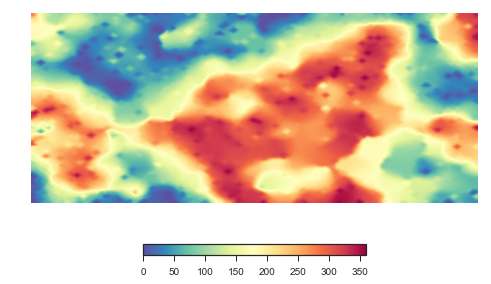
\includegraphics[width=.3\linewidth]{SOM/SOM_OrientationDegrees}}\hfill
	\subfloat[Defectos]{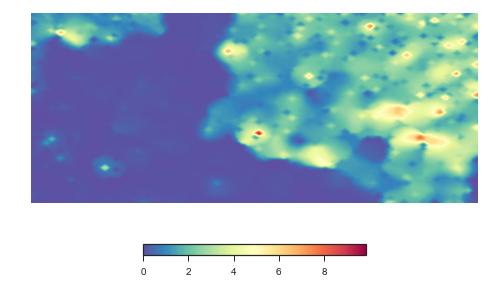
\includegraphics[width=.3\linewidth]{SOM/SOM_DefectosTotales}}
\end{figure}



\begin{figure}[H]
	\caption{\label{SecondSOMASNM}Altitude et défauts lors d'une seconde exécution du réseau de neurones}
	\centering
	\subfloat[ASNM]{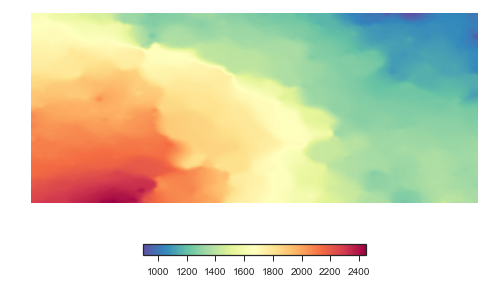
\includegraphics[width=.5\linewidth]{SOM/SOM_ASNM2}}\hfill
	\subfloat[Defectos Totales]{\includegraphics[width=.5\linewidth]{SOM/SOM_DefectosTotales2}}
	\newline

	\centering
	\subfloat[ASNM]{\includegraphics[width=.5\linewidth]{SOM/SOM_ASNM2}}\hfill
	\subfloat[Puntaje Total]{\includegraphics[width=.5\linewidth]{SOM/SOM_PuntajeTotal}}\hfill
	\newline
	\centering 
	\subfloat[Coffee Class Position]{\includegraphics[width=.5\linewidth]{SOM/SOM_Umatrix_Points_Category}}
\end{figure}


\noindent Afin de mieux visualiser la répartition des cafés d'année en année sur la carte SOM, une autre exécution a été réalisée\footnote{Les cartes SOM sont initialisées aléatoirement et les exécutions diffèrent les unes des autres. Il est difficile de sauvegarder l'environnement pour ensuite réaliser d'autres opérations sur les cartes.} et les années affichées. 


\begin{figure}[H]
	\caption{\label{ThirdSOMASNM}Répartition par année et mise en avant des composants intéressants de la SOM}
	\centering
	\subfloat[Umatrix]{\includegraphics[width=.5\linewidth]{SOM/SOM2/umatrix}}\hfill
	\subfloat[Defectos Totales]{\includegraphics[width=.5\linewidth]{SOM/SOM2/umatrix_defectos}}
	\newline
	
	\centering
	\subfloat[Precipitations]{\includegraphics[width=.5\linewidth]{SOM/SOM2/umatrix_prectotalavg}}\hfill
	\subfloat[Year, 2011 (Noir), 2016 (Orange)]{\includegraphics[width=.5\linewidth]{SOM/SOM2/umatrix_year}}\hfill
	\newline
	\centering 
	\subfloat[Coffee Class Position, same as \ref{umatrix_cat}]{\includegraphics[width=.5\linewidth]{SOM/SOM2/umatrix_cat}}
\end{figure}

\newpage
\paragraph{Analyse des cartes}On peut observer que les régions avec beaucoup de précipitations sont aussi celles qui ont le plus de cafés avec peu de points. Lors d'une seconde exécution du réseau on a pu observer une relation proche entre les défauts et l'altitude comme montré sur la figure \ref{SecondSOMASNM}. Cette relation n'était pas clairement visible lors de la première exécution. Le fait est déjà connu que le café qui pousse en altitude est de meilleure qualité cependant ici on remarque que les cafés cultivés aux altitudes les plus hautes sont les plus sujets à une grande quantité de défauts. Les défauts physiques n'interviennent que peu dans la qualité finale du café mais peuvent avoir une influence en cas de mauvais tri. On observe sur la figure \ref{AltPts} que la zone en bas à gauche, là où l'altitude est la plus haute, correspond à une zone possédant peu de cafés ayant eu le score 0 et beaucoup ayant eu des scores entre 85 et 90. Cependant, des cafés ayant un nombre de points de moins de 80 points, en rouge ou compris entre 89 et 85, en bleu, sont présents plus ou moins de manière homogène sur la totalité de la carte, indépendamment de l'altitude. Sur la figure \ref{ThirdSOMASNM} on peut observer que les fortes précipitations sont liées au nombre de défauts mais aussi fortement à l'année. Presque aucun des café de l'année 2011 n'a eu de score compris dans la catégorie 2. 


%TODO trouver le café à 90 points de 2011









\newpage

\section{Apprentissage supervisé}
%Il a été possible ou non de faire de la prédiction, confusion matrix etc
%ce que les méthodes comme random forest ont donné
Le but de cette section est d'analyser la possibilité de prédiction de la qualité des cafés\footnote{La qualité du café fait références aux variables dépendantes citées dans la section \ref{VarDep}.} à l'aide des données climatiques et de qualité de sols à disposition. Les méthodes Random Forest et Partial Least Squares seront utilisées.


\subsection{Random Forest}
 
Cette section présente comment la méthode Random Forest a été utilisée et les résultats produits. 
\subsubsection{Méthode utilisée}
% détails de la méthode, choix pour la cross validation, variables entrée/sortie 
Afin de se faire la meilleure idée possible des possibilités de prédiction, quatre variables de sorties ont été testées. Le nombre total de points (Puntaje Total), l'acidité (Acidez), la douceur (Dulzor) et la catégorie, obtenue d'après le tableau à la section \ref{categoriesCafe}. \\

\noindent La méthode Random Forest du package Caret a été utilisée avec une K-Fold Cross Validation ayant comme paramètre K = 10, répétée 3 fois. 

\begin{lstlisting}[caption={Fonction d'entrainement et de test du modèle avec Random Forest},captionpos=b]
	RFmodelCategory=train(x_cat,y_cat,method="rf",
	tunegrid=tunegrid_cat,
	trControl=trainControl(method="repeatedcv",number=10,repeats=3),
	tuneLength=10,importance = TRUE, proximity=T)
\end{lstlisting}




\newpage
\subsubsection{Résultats de classification}
% Nombre ,graphiques, analyses
En première partie, la tentative de classification avec comme variable de sortie la catégorie. Nous avons pour le modèle:

\begin{itemize}
	\item 490 échantillons \footnote{La totalité des échantillons ont été utilisés ici, y compris ceux possédant 0 points.}
	\item 72 variables indépendantes
	\item 3 classes ("2", "3", "4")
\end{itemize}

Re-échantillonnage des résultats parmi les paramètres de réglage:

\begin{table}[H]
	\centering
	\caption{Réglage du modèle}
	\label{RF_Class_Resampling}
	\begin{tabular}{lll}
		mtry & Accuracy  & Kappa      \\
		2    & 0.4995912 & 0.08462730 \\
		9    & 0.5117305 & 0.10653423 \\
		17   & 0.5062583 & 0.09657805 \\
		25   & 0.5109109 & 0.10608506 \\
		33   & 0.5075520 & 0.10148125 \\
		40   & 0.5014028 & 0.08705477 \\
		48   & 0.5088592 & 0.10056043 \\
		56   & 0.5095934 & 0.10397803 \\
		64   & 0.5081794 & 0.10110968 \\
		72   & 0.5061636 & 0.09829896           
	\end{tabular}
\end{table}

\noindent On observe qu'avec un \textit{mtry}\footnote{À chaque split de l'arbre, l'algorithme va chercher \textit{mtry} variables dans le set. Chaque nouveau split sera composté de \textit{mtry} variables sélectionnées aléatoirement dans le set de donnée principal} de 9, l'\textit{Accuracy} est la meilleure .


\begin{table}[H]
	\centering
	\caption{Les vingt variables les plus importantes par catégorie (sur 72) pour la classification}
	\label{RF_Class_Impvar}
	\begin{tabular}{llll}
		& 2      & 3      & 4      \\
		ASNM      & 60.754 & 38.042 & 100.00 \\
		prec9     & 64.442 & 8.963  & 90.27  \\
		tmin5     & 1.302  & 30.008 & 87.63  \\
		dtr7      & 86.974 & 69.378 & 54.59  \\
		tmean1    & 12.041 & 42.173 & 86.82  \\
		prec10    & 29.188 & 30.604 & 82.33  \\
		tmin4     & 16.840 & 56.842 & 79.80  \\
		tmax5     & 8.655  & 51.687 & 76.56  \\
		tmin1     & 21.357 & 56.763 & 75.76  \\
		tmax4     & 29.270 & 71.631 & 26.10  \\
		tmean2    & 12.710 & 42.159 & 71.51  \\
		tmean5    & 18.301 & 37.089 & 70.87  \\
		dtr5      & 16.198 & 70.822 & 39.11  \\
		tmax8     & 9.814  & 50.375 & 70.72  \\
		dtr8      & 10.785 & 43.304 & 70.20  \\
		tmax6     & 18.386 & 68.704 & 51.16  \\
		prec6     & 40.057 & 25.298 & 68.17  \\
		DtrTotal  & 13.864 & 67.471 & 36.17  \\
		Cascajoso & 42.708 & 54.120 & 65.70  \\
		tmax10    & 6.866  & 45.774 & 65.59  \\
		&        &        &        \\
		&        &        &       
	\end{tabular}
\end{table}

\noindent Enfin après avoir construit le modèle, on peut le valider avec nos données de test. Nous obtenons les résultats suivants: 


\begin{figure}[H]
	\centering
	\includegraphics[scale=0.4]{../../Bachelor_Thesis_2017_Sources/Notebook/R/Projects/BachelorThesis/RF_models_perfs/ConfusionMatrix_RF_Classification_Result}
	\caption{Matrice de confusion de la classification avec Random Forest}
	\label{fig:confusionmatrixrfclassificationresult}
\end{figure}

\begin{minipage}{\linewidth}
	
	\begin{lstlisting}[showstringspaces=false,language=R, caption={Test du modèle de classification},captionpos=b]
		
		          Reference
	Prediction  2  3  4
		2   2  1  2
		3   9 50 50
		4   3 43 47
		
		
		Overall Statistics
		
		Accuracy : 0.4783          
		95% CI : (0.4085, 0.5486)
		No Information Rate : 0.4783          
		P-Value [Acc > NIR] : 0.52732         
		
		Kappa : 0.0416          
		Mcnemar's Test P-Value : 0.06796         
		
 Statistics by Class:
		
                      Class: 2 Class: 3 Class: 4
Sensitivity          0.142857   0.5319   0.4747
Specificity          0.984456   0.4779   0.5741
Pos Pred Value       0.400000   0.4587   0.5054
Neg Pred Value       0.940594   0.5510   0.5439
Prevalence           0.067633   0.4541   0.4783
Detection Rate       0.009662   0.2415   0.2271
Detection Prevalence 0.024155   0.5266   0.4493
Balanced Accuracy    0.563657   0.5049   0.5244
	\end{lstlisting}
\end{minipage}





%-------------------------------------------------------------------------

\newpage
\subsubsection{Régression sur la variable dépendante \textit{Puntaje Total}}
\noindent Notre modèle contient: 
\begin{itemize}
	\item 448 échantillons
	\item 72 variables indépendantes
\end{itemize}


\begin{table}[H]
	\centering
	\caption{Réglage du modèle}
	\label{RF_Total_Resampling}
	\begin{tabular}{llll}
		mtry & RMSE     & Rsquared     \\
		2    & 6.033466 & 0.03056280   \\
		9    & 6.063304 & 0.03686526   \\
		17   & 6.042679 & 0.04446260   \\
		25   & 6.056445 & 0.04747083   \\
		33   & 6.064986 & 0.05062423   \\
		40   & 6.052046 & 0.05279225   \\
		48   & 6.076724 & 0.05268180   \\
		56   & 6.084703 & 0.05124400   \\
		64   & 6.066546 & 0.05294682   \\
		72   & 6.079099 & 0.05567081    
	\end{tabular}
\end{table}

\noindent On observe qu'avec un \textit{mtry} de 2, la RMSE est la plus petite. Cependant, une fois testé le modèle donne l'erreur suivante: RMSE = 7.1726 et Rsquared = 0.00431. 


\begin{figure}[H]
	\centering
	\includegraphics[width=0.9\linewidth]{../../Bachelor_Thesis_2017_Sources/Notebook/R/Projects/BachelorThesis/RF_models_perfs/modele_Total_Regression}
	\caption{Performances de la régression pour la variable \textit{Puntaje Total}}
	\label{fig:modeletotalregression}
\end{figure}

\begin{minipage}{\linewidth}
	
	\begin{lstlisting}[showstringspaces=false,language=R, caption={Test du modèle de classification},captionpos=b]
	Call:
	randomForest(x = x, y = y, mtry = param$mtry, 
	importance = TRUE,
	proximity = ..3, tunegrid = ..1) 
	
	Type of random forest: regression
	Number of trees: 500
	No. of variables tried at each split: 2
	
	Mean of squared residuals: 38.38491
	% Var explained: -9.59
	
	\end{lstlisting}
\end{minipage}


\begin{table}[H]
	\centering
	\caption{Les 20 variables les plus importantes du modèle.}
	\label{RF_Total_Varimp}
	\begin{tabular}{ll}
		& Overall \\
		tmean2       & 100.00  \\
		tmax6        & 99.28   \\
		tmean4       & 96.71   \\
		tmax2        & 94.71   \\
		tmax5        & 92.77   \\
		PrecTotalAvg & 90.81   \\
		tmax4        & 88.96   \\
		dtr4         & 88.89   \\
		tmin2        & 87.82   \\
		DtrTotal     & 87.43   \\
		tmin3        & 87.25   \\
		tmin5        & 86.97   \\
		tmean1       & 86.93   \\
		tmean8       & 85.72   \\
		tmax8        & 85.34   \\
		TminTotalAvg & 84.71   \\
		dtr2         & 84.71   \\
		tmean10      & 84.42   \\
		tmin1        & 83.93   \\
		prec10       & 83.85  
	\end{tabular}
\end{table}



\begin{figure}[H]
	\centering
	\includegraphics[width=0.7\linewidth]{../../Bachelor_Thesis_2017_Sources/Notebook/R/Projects/BachelorThesis/RF_models_perfs/Pred_PuntajeTotal}
	\caption{Comparaison des prédiction et des valeurs actuelle pour la variable \textit{Puntaje Total}}
	\label{fig:predpuntajetotal}
\end{figure}



%-----------------------------------------------------------------------


\newpage
\subsubsection{Régression sur la variable dépendante \textit{Acidez}}
\noindent Notre modèle contient: 
\begin{itemize}
	\item 448 échantillons
	\item 72 variables indépendantes
\end{itemize}


\begin{table}[H]
	\centering
	\caption{Réglage du modèle}
	\label{RF_Acidez_Resampling}
	\begin{tabular}{llll}
	    mtry & RMSE      & Rsquared   \\
	    2    & 0.5523984 & 0.07780696 \\
	    9    & 0.5587745 & 0.07205180 \\
	    17   & 0.5591882 & 0.07332069 \\
	    25   & 0.5614777 & 0.07128568 \\
	    33   & 0.5601199 & 0.07188263 \\
	    40   & 0.5602361 & 0.07391410 \\
	    48   & 0.5608331 & 0.07075389 \\
	    56   & 0.5599010 & 0.07333161 \\
	    64   & 0.5604395 & 0.07236162 \\
	    72   & 0.5607297 & 0.07082403
	\end{tabular}
\end{table}

\noindent On observe qu'avec un \textit{mtry} de , la RMSE est la plus petite. Cependant, une fois entrainé le modèle donne l'erreur suivante: RMSE = 0.5587  et Rsquared = 0.0261. 

\begin{figure}[H]
	\centering
	\includegraphics[width=0.9\linewidth]{../../Bachelor_Thesis_2017_Sources/Notebook/R/Projects/BachelorThesis/RF_models_perfs/modele_Acidez_regression}
	\caption{Performances de la régression pour la variable \textit{Acidez}}
	\label{fig:modeleacidezregression}
\end{figure}


\begin{minipage}{\linewidth}
	
	\begin{lstlisting}[showstringspaces=false,language=R, caption={Test du modèle de classification},captionpos=b]
	Call:
	randomForest(x = x, y = y, mtry = param$mtry, 
	importance = TRUE,      
	proximity = ..3, tunegrid = ..1) 
	Type of random forest: regression
	Number of trees: 500
	No. of variables tried at each split: 2
	
	Mean of squared residuals: 0.3157974
	% Var explained: -1.63
	\end{lstlisting}
\end{minipage}


\begin{table}[H]
	\centering
	\caption{Les 20 variables les plus importantes du modèle.}
	\label{RF_Acidez_Varimp}
	\begin{tabular}{ll}
	 & Overall \\
	 dtr10         & 100.00  \\
	 tmin9         & 98.16   \\
	 tmean3        & 96.84   \\
	 tmax8         & 96.40   \\
	 tmax7         & 94.54   \\
	 tmax6         & 93.25   \\
	 tmin3         & 92.78   \\
	 TmeanTotalAvg & 90.41   \\
	 DtrTotalAvg   & 89.54   \\
	 tmax3         & 89.17   \\
	 TmaxTotalAvg  & 88.40   \\
	 tmax5         & 87.07   \\
	 tmax10        & 85.38   \\
	 TminTotalAvg  & 84.12   \\
	 dtr8          & 83.90   \\
	 tmean10       & 83.73   \\
	 tmin5         & 83.27   \\
	 tmax1         & 82.81   \\
	 tmean4        & 82.49   \\
	 tmean9        & 81.66  
	\end{tabular}
\end{table}

\begin{figure}[H]
	\centering
	\includegraphics[width=0.7\linewidth]{../../Bachelor_Thesis_2017_Sources/Notebook/R/Projects/BachelorThesis/RF_models_perfs/Pred_ACidez}
	\caption{Comparaison des prédiction et des valeurs actuelle pour la variable \textit{Acidez}}
	\label{fig:predacidez}
\end{figure}


%TODO plot acidez vs altitude ou pas
%LA RMSE est bonne ici -> regarder Rsquared, car pas dépendent de l'unité, si proche de 1 c'est bon sinon c'est dela merde ->  c'est toujours de la merde -> commentj'aie u peur d'un coup !


%-----------------------------------------------------------------------


\newpage
\subsubsection{Régression sur la variable dépendante \textit{Dulzor}}
\noindent Notre modèle contient: 
\begin{itemize}
	\item 439 échantillons
	\item 72 variables indépendantes
\end{itemize}


\begin{table}[H]
	\centering
	\caption{Réglage du modèle}
	\label{RF_Dulzor_Resampling}
	\begin{tabular}{llll}
	mtry & RMSE      & Rsquared   \\
	2    & 0.7996682 & 0.02423378 \\
	9    & 0.8030381 & 0.03690104 \\
	17   & 0.8082138 & 0.04453890 \\
	25   & 0.8112174 & 0.04482055 \\
	33   & 0.8141780 & 0.04452465 \\
	40   & 0.8163036 & 0.04853452 \\
	48   & 0.8187376 & 0.04858482 \\
	56   & 0.8211659 & 0.04628629 \\
	64   & 0.8209675 & 0.04722086 \\
	72   & 0.8226232 & 0.04976240
	\end{tabular}
\end{table}

\noindent On observe qu'avec un \textit{mtry} de 2, la RMSE est la plus petite. Cependant, une fois entrainé le modèle donne l'erreur suivante: RMSE = 0.8747  et Rsquared = 0.0009. 

\begin{figure}[H]
	\centering
	\includegraphics[width=0.9\linewidth]{../../Bachelor_Thesis_2017_Sources/Notebook/R/Projects/BachelorThesis/RF_models_perfs/modele_dulzor_regression}
	\caption{Performances de la régression pour la variable \textit{Dulzor}}
	\label{fig:modeledulzorregression}
\end{figure}



\begin{minipage}{\linewidth}
	
	\begin{lstlisting}[showstringspaces=false,language=R, caption={Test du modèle de classification},captionpos=b]
Call:
randomForest(x = x, y = y, mtry = param$mtry, 
importance = TRUE,      
proximity = ..3, tunegrid = ..1) 
Type of random forest: regression
Number of trees: 500
No. of variables tried at each split: 2

Mean of squared residuals: 0.7230219
% Var explained: -9.25
	\end{lstlisting}
\end{minipage}


\begin{table}[H]
	\centering
	\caption{Les 20 variables les plus importantes du modèle.}
	\label{RF_Dulzor_Varimp}
	\begin{tabular}{ll}
              & Overall \\
dtr4          & 100.00  \\
tmax4         & 99.29   \\
tmax9         & 96.55   \\
tmin4         & 93.13   \\
tmean4        & 92.17   \\
TmaxTotal     & 91.49   \\
tmin5         & 90.85   \\
TmeanTotal    & 90.64   \\
prec6         & 89.90   \\
tmin2         & 89.84   \\
dtr10         & 89.69   \\
tmax6         & 89.17   \\
tmax5         & 87.47   \\
tmax7         & 87.16   \\
dtr8          & 87.15   \\
tmax2         & 86.37   \\
dtr2          & 86.23   \\
tmean1        & 85.78   \\
TmeanTotalAvg & 85.08   \\
DtrTotal      & 84.98
	\end{tabular}
\end{table}


\begin{figure}[H]
	\centering
	\includegraphics[width=0.7\linewidth]{../../Bachelor_Thesis_2017_Sources/Notebook/R/Projects/BachelorThesis/RF_models_perfs/Pred_Dulzor}
	\caption{Comparaison des prédiction et des valeurs actuelle pour la variable \textit{Dulzor}}
	\label{fig:preddulzor}
\end{figure}


\newpage


%TODO Footnote pour kappa
\paragraph{Discussion des résultats pour Random Forest}
Avec une \textit{accuracy} de seulement 0.47  (47\% d'échantillons classés correctement) et un test de Kappa d'uniquement 0.0416, la classification à l'aide de Random Forest ne semble pas fiable avec les données en notre possession. \\

\noindent Pour mesurer la qualité de la régression, nous utiliserons comme mesure le coefficient $r^2$ fournit par les résultats de Random Forest. Plus le coefficient s'approche de $1$ plus la variation totale des sorties prédites par le modèle est faible et donc plus le modèle est bon. Les résultats obtenus avec les 3 variables de sortie différentes sont les suivants: \\


\begin{itemize}
	\item Puntaje Total: $r^2 = 0.00431$
	\item Acidez: $r^2 = 0.0261$
	\item Dulzor: $r^2 = 0.0009$
\end{itemize} 












%TODO finir RF et parler de RF avec les variables sans variance etc
\subsection{Random Forest avec variables à haute variabilité}
Afin de tester le modèle sans données inutilement redondantes et fortement corrélées, un second modèle Random Forest a été entrainé avec les variables indépendantes qui avaient un taux de variabilité supérieur à un certain niveau. Le premier niveau a été placé à $10$, ce qui a pour effet de ne garder que $25$ variables. Le second a été placé à $20$, ce qui a pour effet de ne garder que $21$ variables. Les résultats se sont avérés tout aussi imprécis, voir par exemple les résultats de prédiction sur la figure \ref{fig:rfptotalvariability10} avec le seuil à 10 pour la variable \textit{Puntaje Total} et sur la figure \ref{fig:rfptotalvariability20} avec le seuil à 20. Les cafés ayant un total de zéro points ont ici été gardés afin d'observer une éventuelle prédiction correspondante. Sur la figure \ref{fig:rfptotalvariability10} on peut observer qu'un des café ayant zéro points a été prédit à moins de 40 points. Les variables montrée dans le tableau \ref{tab:variability10Variables} sont celles utilisées pour créer le modèle avec un seuil de 10. On peut voir que les précipitations ont une grande importance et cela rejoint l'idée observée dans la section \ref{SOM} que la quantité de précipitations est importante pour la qualité du grain, cependant cela ne permet que d'avoir une approximation de la quantité de défauts physique du grain et non sur la qualité générale. 

\begin{figure}[H]
	\centering
	\includegraphics[width=0.7\linewidth]{../../Bachelor_Thesis_2017_Sources/Notebook/R/Projects/BachelorThesis/RF_models_perfs/RF_PTotal_Variability10}
	\caption{Prédiction du total de points avec 25 variables indépendantes}
	\label{fig:rfptotalvariability10}
\end{figure}
\begin{figure}[H]
	\centering
	\includegraphics[width=0.7\linewidth]{../../Bachelor_Thesis_2017_Sources/Notebook/R/Projects/BachelorThesis/RF_models_perfs/RF_PTotal_Variability20}
	\caption{Prédiction du total de points avec 21 variables indépendantes}
	\label{fig:rfptotalvariability20}
\end{figure}





\begin{table}[H]
	\centering
	\caption{Variables à haute variabilité avec un coefficient de variabilité supérieur à 10}
	\label{tab:variability10Variables}
	\begin{tabular}{lll}
		& \%IncMSE   & IncNodePurity \\
		ASNM           & 5.0408727  & 15044.3045    \\
		Luminosidad    & 5.4787179  & 3642.4806     \\
		prec1          & 7.6033403  & 11395.8391    \\
		prec2          & 8.4894841  & 12991.3588    \\
		prec3          & 9.6477012  & 14018.6199    \\
		prec4          & 7.6742913  & 16432.9873    \\
		prec5          & 8.5170477  & 13554.8590    \\
		prec6          & 9.3037427  & 14994.6836    \\
		prec7          & 7.3229410  & 14325.6941    \\
		prec8          & 9.0394682  & 13509.3978    \\
		prec9          & 9.6867243  & 13287.9725    \\
		prec10         & 12.0962566 & 17472.3424    \\
		dtr5           & 10.2926692 & 16738.1273    \\
		dtr10          & 9.1992584  & 15261.9880    \\
		PrecTotal      & 12.0991208 & 15483.9130    \\
		PrecTotalAvg   & 11.6456487 & 13780.0364    \\
		OrientationNum & 2.4731816  & 10925.6272    \\
		Slope          & 0.1353807  & 15492.9382    \\
		org\_avg       & 2.7056077  & 6520.6197     \\
		Franco         & 1.5936970  & 1931.0307     \\
		Arcilloso      & -2.9621275 & 1746.0451     \\
		Limoso         & 2.7839655  & 1631.1038     \\
		Arenoso        & -1.5199547 & 831.4292      \\
		Cascajoso      & -0.5423810 & 2330.3915    
	\end{tabular}
\end{table}














\newpage

\subsection{Partial Least Squares}
% analyser les résultats de prédiction ainsi que les corrélation fournies par PLS - au vus des résultats et de la corrélation entre les variables de sorties pas besoind 'utiliser MBPLS ça serait une perte de temps
Cette méthode utilise à la fois le principe de régression et d'analyse en composante principale (PCA ou ACP). La méthode \textit{plsreg1} de R fournit en retour plusieurs objets dont les corrélation entre variable dont la représentation graphique permet de visualiser aisément où se placent les variables de sorties choisie. 

\begin{figure}[H]
	\centering
	\includegraphics[scale=0.5]{../../Bachelor_Thesis_2017_Sources/Notebook/R/Projects/BachelorThesis/PLS/CircleOfCorrelationPuntajeTotal}
	\caption{Représentation des corrélations entre les variables indépendantes et la variable dépendante \textit{Puntaje Total}}
	\label{fig:circleofcorrelationpuntajetotal}
\end{figure}
 
\begin{figure}[H]
	\centering
	\includegraphics[scale=0.5]{../../Bachelor_Thesis_2017_Sources/Notebook/R/Projects/BachelorThesis/PLS/CircleOfCorrelationAcidez}
	\caption{Représentation des corrélations entre les variables indépendantes et la variable dépendante \textit{Acidez}}
	\label{fig:circleofcorrelationacidez}
\end{figure}

\begin{figure}[H]
	\centering
	\includegraphics[scale=0.5]{../../Bachelor_Thesis_2017_Sources/Notebook/R/Projects/BachelorThesis/PLS/CircleOfCorrelationDulzor}
	\caption{Représentation des corrélations entre les variables indépendantes et la variable dépendante \textit{Dulzor}}
	\label{fig:circleofcorrelationdulzor}
\end{figure}


\subsubsection{Analyse des résultats}

La prédiction avec Partial Least Squares ne donne pas de résultats plus convainquant que Random Forest. Cependant et afin de mitiger ces résultats, la méthode n'a pas été exploitée avec son plein potentiel car un seul block de donnée à été utilisé (la totalité des variables indépendantes) alors que PLS et Multiblock PLS peuvent éventuellement être amélioré en réglant les paramètres plus finement. 

\begin{figure}[H]
	\centering
	\includegraphics[width=0.7\linewidth]{../../Bachelor_Thesis_2017_Sources/Notebook/R/Projects/BachelorThesis/PLS/ComparisonOfResponsesPuntajeTotal}
	\caption{Comparaison des prédiction et des valeurs actuelle pour la variable Puntaje Total}
	\label{fig:comparisonofresponsespuntajetotal}
\end{figure}


\begin{figure}[H]
	\centering
	\includegraphics[width=0.7\linewidth]{../../Bachelor_Thesis_2017_Sources/Notebook/R/Projects/BachelorThesis/PLS/ComparisonOfResponsesAcidez}
	\caption{Comparaison des prédiction et des valeurs actuelle pour la variable Acidez}
	\label{fig:comparisonofresponsesacidez}
\end{figure}



\begin{figure}[H]
	\centering
	\includegraphics[width=0.7\linewidth]{../../Bachelor_Thesis_2017_Sources/Notebook/R/Projects/BachelorThesis/PLS/ComparisonOfResponsesDulzor}
	\caption{Comparaison des prédiction et des valeurs actuelle pour la variable Dulzor}
	\label{fig:comparisonofresponsesdulzor}
\end{figure}



















